%%%%%%%%%%%%%%%%%%%%%%%%%%%%%%%%%%%%%%%%%%%%%%%%%%%%%%%%%%%%
% CHAPTER 3 – REQUIREMENT ANALYSIS
%%%%%%%%%%%%%%%%%%%%%%%%%%%%%%%%%%%%%%%%%%%%%%%%%%%%%%%%%%%%

\chapter{Requirement Analysis}

%===========================================================
\section{Introduction to Requirement Analysis}
%===========================================================

This chapter presents a structured and formal specification of system requirements for the Lets Go Ride Sharing App ride-sharing application. The purpose of this chapter is to clearly define what the system shall accomplish before proceeding to the system design phase. The requirements documented in this chapter serve as a contractual foundation for implementation, validation, and system testing.

The requirement analysis includes requirement elicitation techniques, identification of stakeholders, use case modeling, functional requirements, non-functional requirements, and external interface requirements. All requirements are written in measurable and testable format using standard requirement engineering principles.

%===========================================================
\section{Requirement Elicitation Techniques}
%===========================================================

This section describes the techniques used to gather and refine system requirements. Requirement elicitation ensures alignment between stakeholder expectations and system capabilities.

Requirements for the Lets Go Ride Sharing App project were identified using the following techniques:

\begin{itemize}
    \item \textbf{Stakeholder interviews} with potential drivers, passengers, and administrators to capture user expectations, pain points, and desired features.
    \item \textbf{Literature review} of existing ride-sharing platforms (BlaBlaCar, InDrive, Bykea) and academic research on carpooling systems.
    \item \textbf{Analysis of existing solutions} to identify functional gaps, such as lack of route-based matching and cultural preferences.
    \item \textbf{Dataset examination} for the machine learning module, studying travel patterns and user behavior to define recommendation and recommendation evaluation features.
    \item \textbf{Observation of workflow processes} in current transportation services to understand manual verification, payment handling, and dispute resolution needs.
\end{itemize}

%===========================================================
\section{User Classes and Characteristics}
%===========================================================

This section defines the different user categories interacting with the Lets Go Ride Sharing App system. Each user class is described along with responsibilities, access privileges, and typical technical proficiency. This classification supports role-based access control and requirement mapping.

% keep table Table 3.1: User Classes and Characteristics as it is

\begin{table}[htbp]
\centering
\caption{User Classes and Characteristics}
\begin{tabularx}{\textwidth}{|p{3cm}|X|p{3cm}|}
\hline
\rowcolor{lightgray!30}
\textbf{User Class} & \textbf{Description} & \textbf{Technical Level} \\
\hline
Admin & Manages user verification, dispute resolution, financial analytics, and system configuration via a web-based Admin panel. & Advanced \\
\hline
Driver & Creates rides, manages vehicles, accepts bookings, coordinates with passengers, and completes trips. Must undergo document verification. & Intermediate \\
\hline
Passenger & Searches and books rides, communicates with drivers, makes payments, and provides ratings. & Basic \\
\hline
External System & Third-party services such as Maps API, Notification Service (FCM, SMS, email), and LLM API for chatbot integration. & Technical \\
\hline
\end{tabularx}
\end{table}

The system boundary includes all internal modules, user interfaces, data processing components, and integrated third-party services (Maps, Notifications, LLM). External entities interact with the system via well-defined APIs.

%===========================================================
\section{Use Case Model}
%===========================================================

The use case model represents high-level system interactions between actors and system functionalities. It defines system boundaries and captures functional behaviour from a user perspective.

%-----------------------------------------------------------------
\subsection{Use Case Diagram}
%-----------------------------------------------------------------

The Lets Go Ride Sharing App system includes 25 use cases that span registration, vehicle availability, driver–passenger interactions, ride creation, booking, ride execution, safety and dispute handling, ML recommendations, chatbot support, and manual payment flows. The diagrams in the repository illustrate the system and thematic groupings.

\begin{figure}[H]
    \centering
    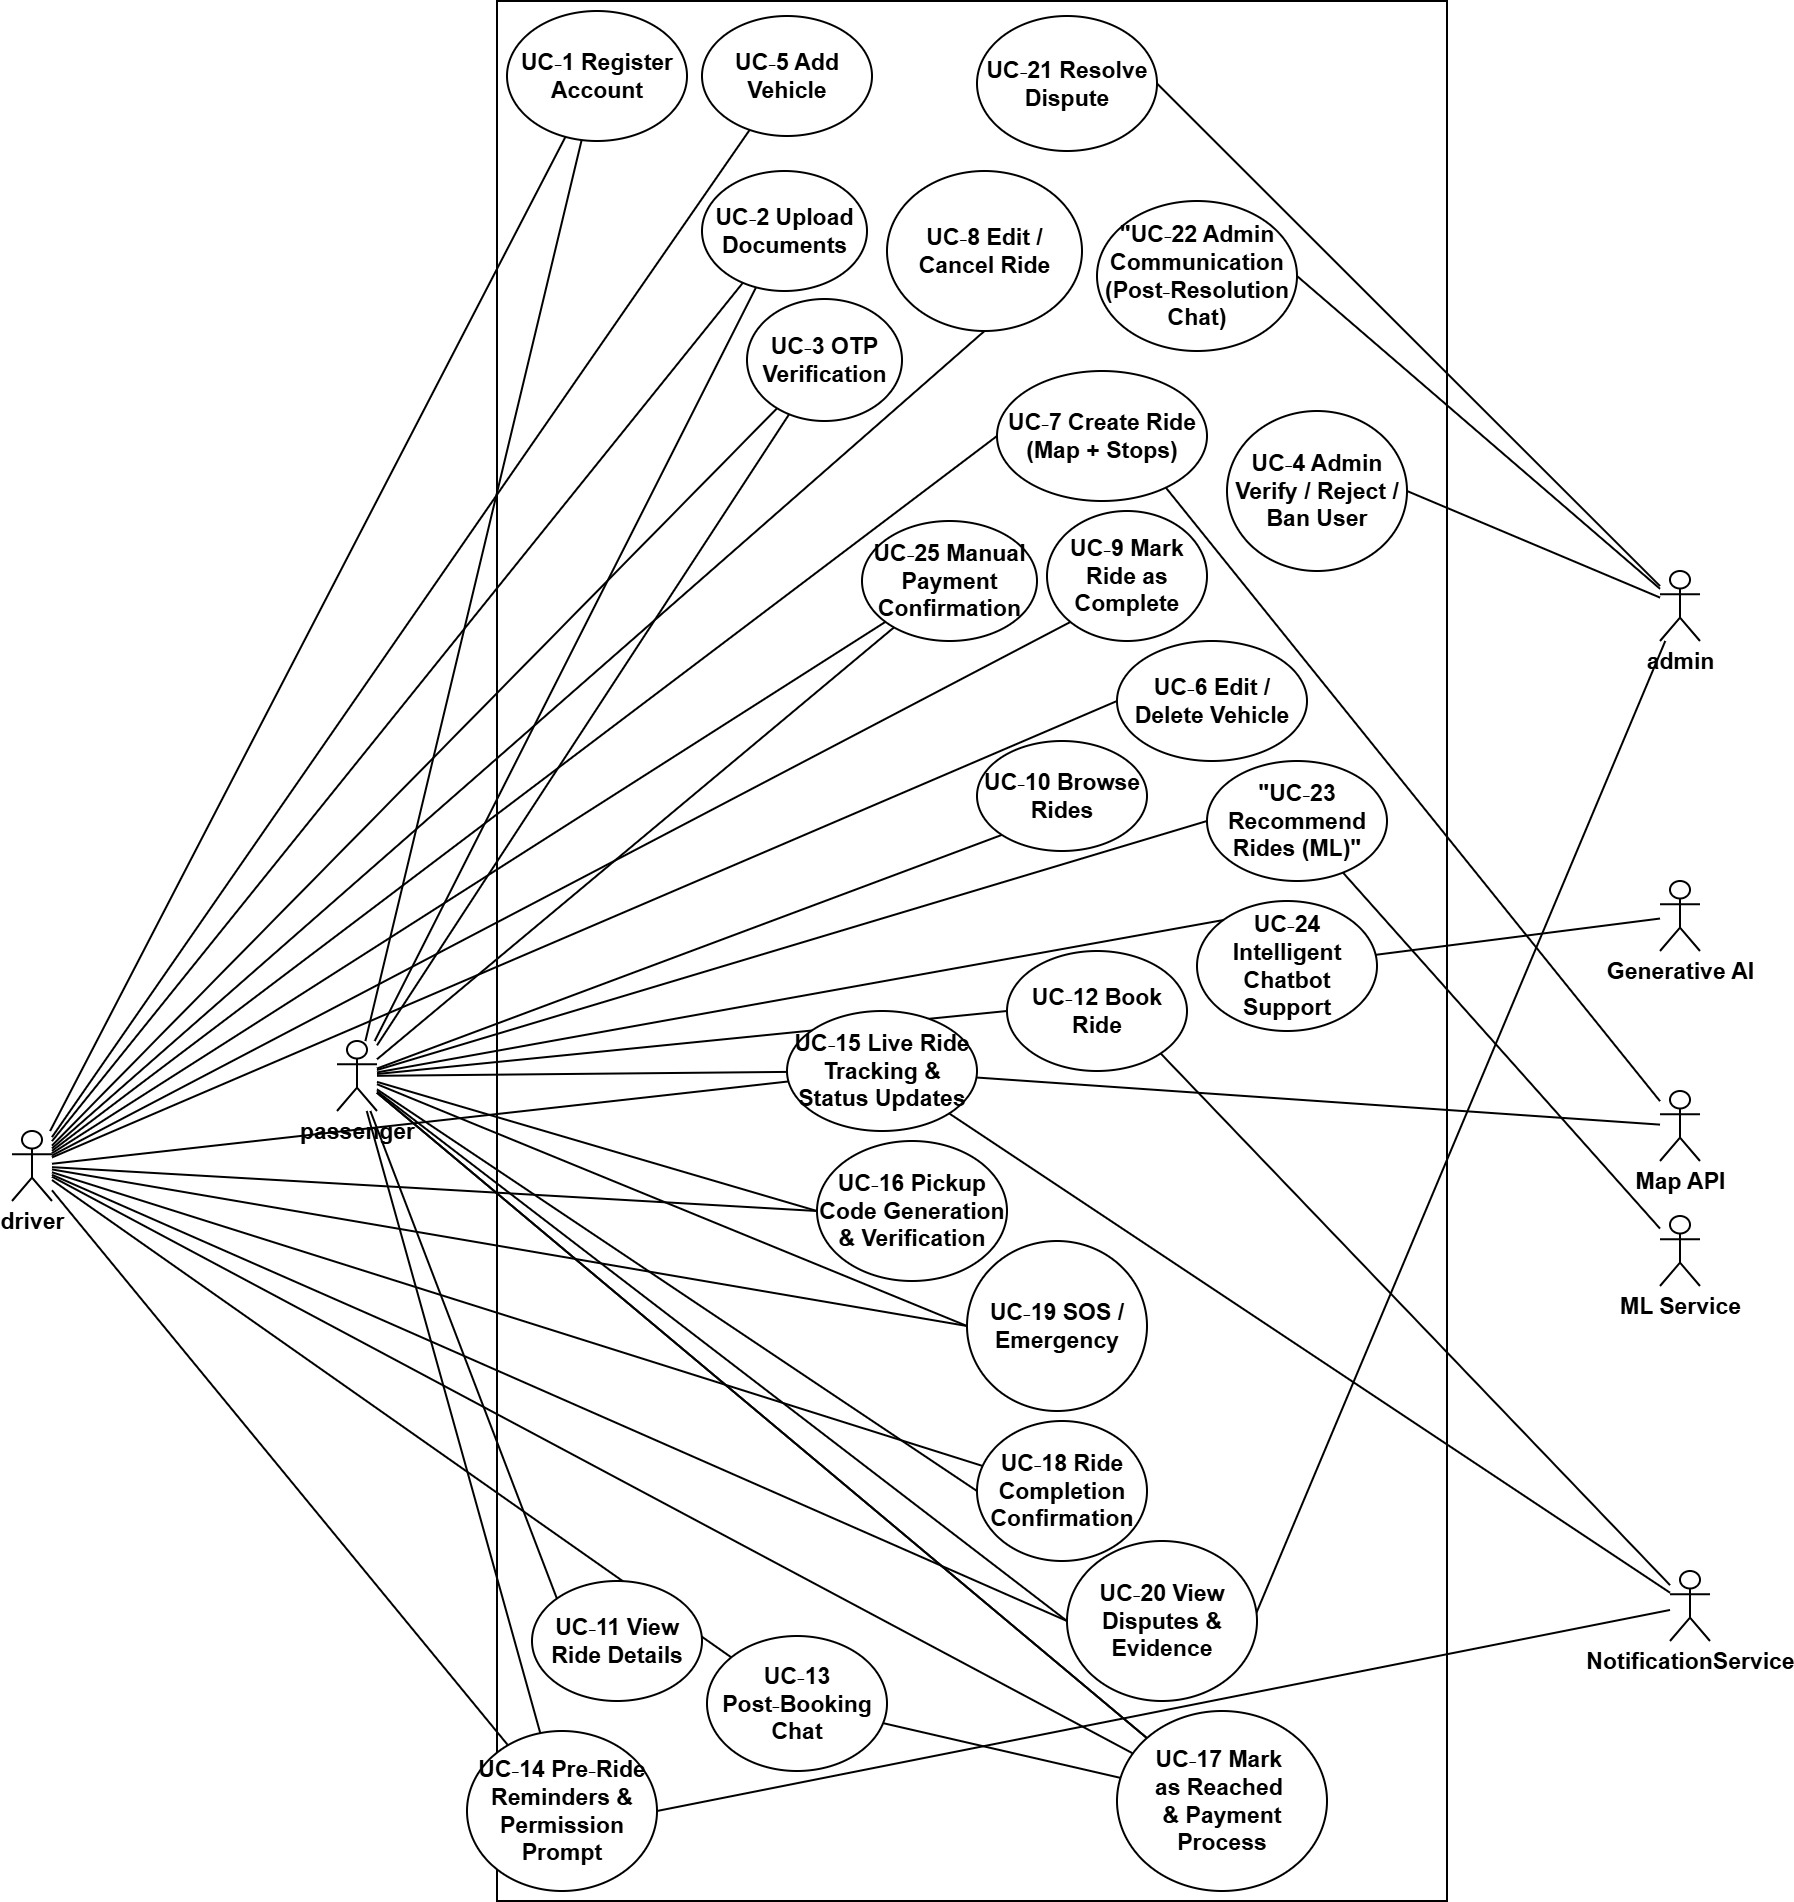
\includegraphics[width=\textwidth,keepaspectratio]{assets/master_uc.jpg}
    \caption{Master Use Case Diagram for the Lets Go Ride Sharing App system, covering all use cases and actor interactions.}
    \label{fig:master_uc}
\end{figure}

\begin{figure}[H]
    \centering
    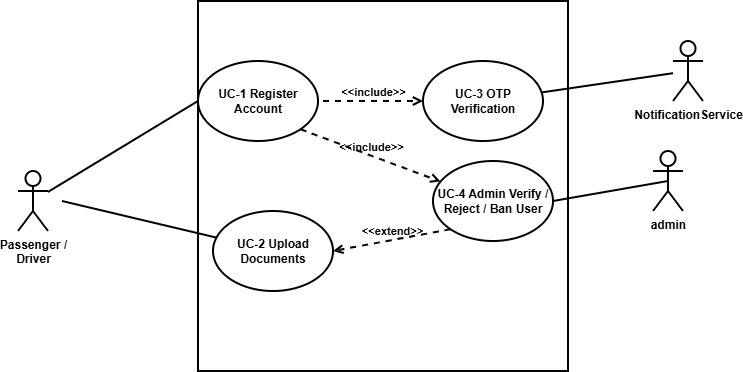
\includegraphics[width=0.8\textwidth,keepaspectratio,height=0.45\textheight]{assets/reg_verification_uc.jpg}
    \caption{Registration and Verification Theme: flow from account creation and multi-channel OTP verification to manual Admin identity approval.}
    \label{fig:registration_uc}
\end{figure}

\begin{figure}[H]
    \centering
    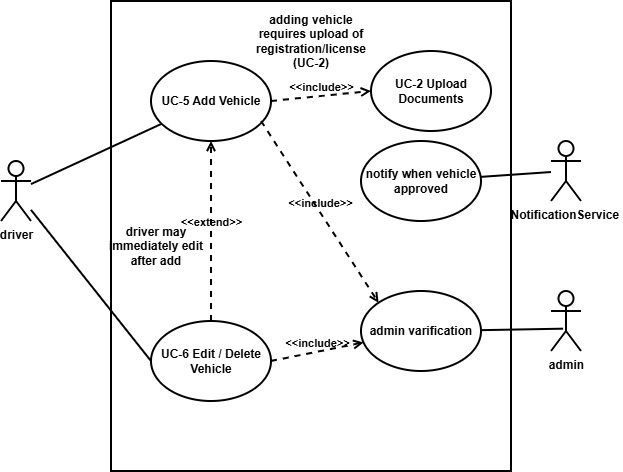
\includegraphics[width=0.8\textwidth,keepaspectratio,height=0.45\textheight]{assets/vehicle_management_uc.jpg}
    \caption{Vehicle Management: driver vehicle registration lifecycle and maintenance considerations.}
    \label{fig:vehicle_uc}
\end{figure}

\begin{figure}[H]
    \centering
    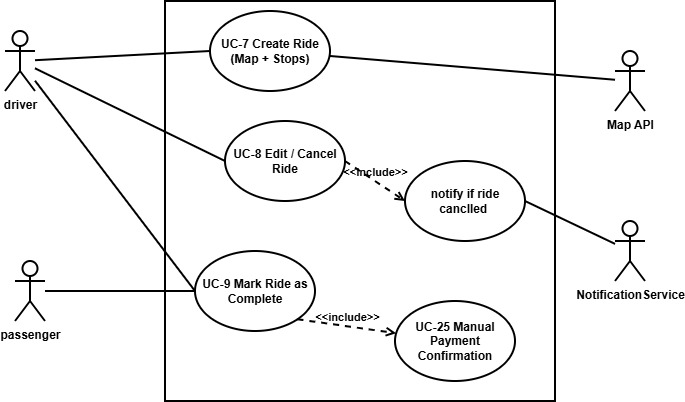
\includegraphics[width=0.8\textwidth,keepaspectratio,height=0.45\textheight]{assets/ride_management_uc.jpg}
    \caption{Ride Management: driver-side ride lifecycle from route creation to completion.}
    \label{fig:ride_mgmt_uc}
\end{figure}

\begin{figure}[H]
    \centering
    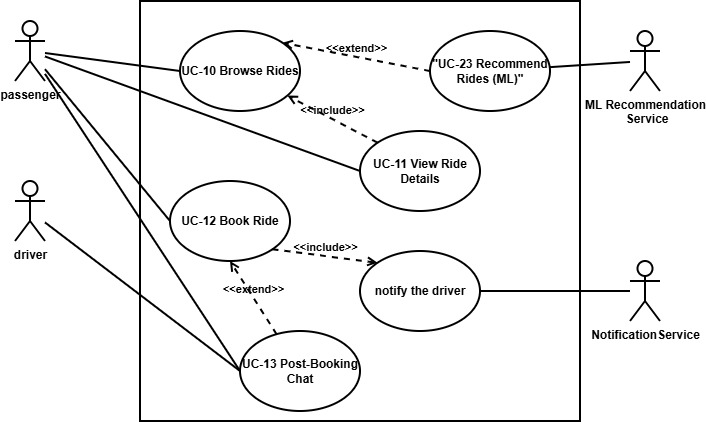
\includegraphics[width=0.8\textwidth,keepaspectratio,height=0.45\textheight]{assets/discovery_booking_uc.jpg}
    \caption{Discovery and Booking: passenger search, seat lock mechanism, and post-booking coordination.}
    \label{fig:booking_uc}
\end{figure}

\clearpage
\begin{figure}[H]
    \centering
    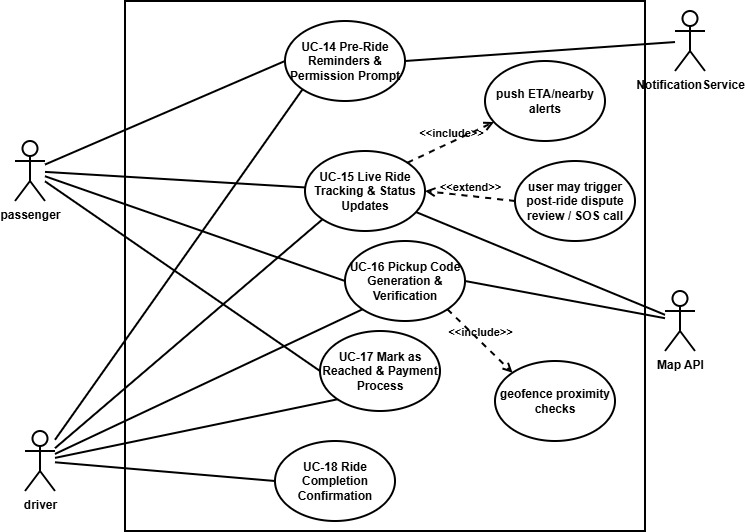
\includegraphics[width=0.8\textwidth,keepaspectratio,height=0.4\textheight]{assets/ride_execution_uc.jpg}
    \caption{Ride Execution Phase: live GPS tracking, geofenced pickup OTP verification, and arrival confirmations.}
    \label{fig:execution_uc}
\end{figure}

\begin{figure}[H]
    \centering
    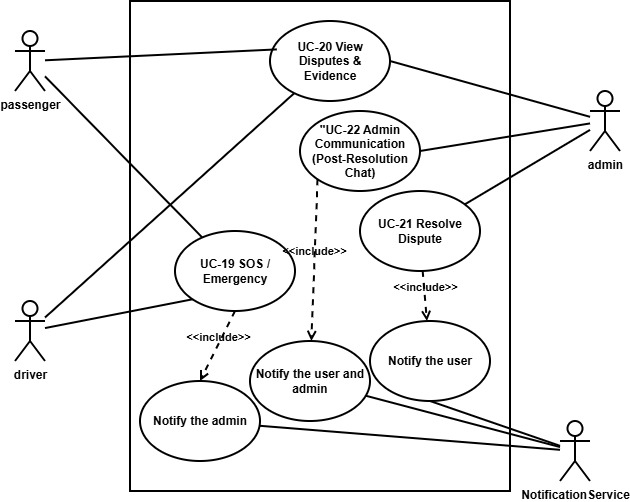
\includegraphics[width=0.8\textwidth,keepaspectratio,height=0.4\textheight]{assets/safety_disputes_uc.jpg}
    \caption{Safety and Disputes: SOS alerts, emergency escalation, and Admin audit workflows.}
    \label{fig:safety_uc}
\end{figure}

\clearpage
\begin{figure}[H]
    \centering
    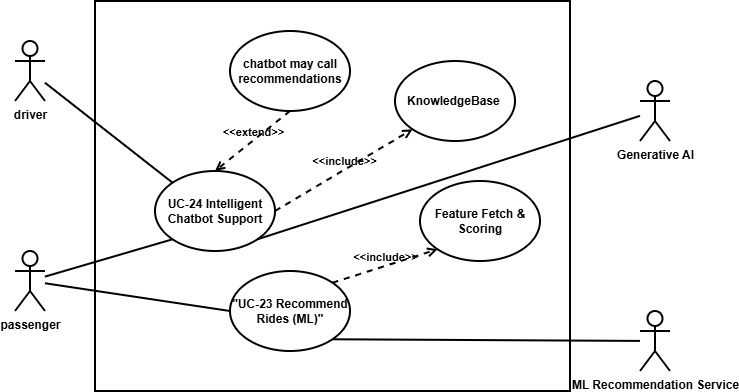
\includegraphics[width=0.8\textwidth,keepaspectratio,height=0.4\textheight]{assets/ml_chatbot_uc.jpg}
    \caption{AI/ML Features: content-based ride recommendations and generative AI support.}
    \label{fig:ai_uc}
\end{figure}

\begin{figure}[H]
    \centering
    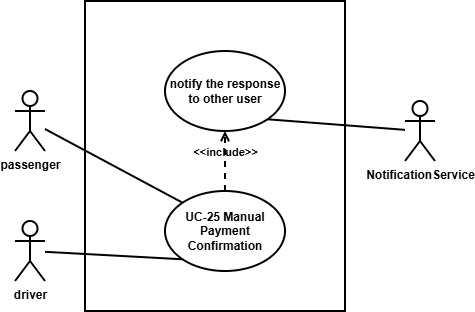
\includegraphics[width=0.8\textwidth,keepaspectratio,height=0.4\textheight]{assets/payment_uc.jpg}
    \caption{Manual Payment Flow: two-step verification for external transfers (Cash/Bank/QR).}
    \label{fig:payment_uc}
\end{figure}

\clearpage

%-----------------------------------------------------------------
\subsection{Use Case Descriptions}
%-----------------------------------------------------------------

This section provides detailed tabular specifications of all major use cases. These use cases form the basis for deriving functional requirements and are organised by thematic modules.

%============================================================================
\subsubsection{Registration \& Verification (UC-1 to UC-4)}
%============================================================================

% ============================================================================
% Use Case UC-1: Register Account
% ============================================================================
\begin{longtable}{|>{\raggedright\arraybackslash}p{4cm}|>{\raggedright\arraybackslash}p{11cm}|}
\caption{UC-1: Register Account}
\label{tab:uc-1} \\
\hline
\rowcolor{lightgray!30}
\textbf{Field} & \textbf{Value} \\
\hline
\endfirsthead
\hline
\rowcolor{lightgray!30}
\textbf{Field} & \textbf{Value} \\
\hline
\endhead
\hline
\endfoot
\hline
\endlastfoot
Use Case ID & UC-1 \\
\hline
Use Case Name & Register Account \\
\hline
Actors & \textbf{Primary Actor:} Unverified User \\
& \textbf{Secondary Actors:} Notification Service (email/SMS), Admin (implicit actor for later verification), Chatbot (optional help) \\
\hline
Description & An Unverified User registers a new account by supplying personal information and optional driver/bank details, uploads required documents (profile photo, live photo, CNIC front/back, driving license if applicable), receives OTPs via email and SMS, and completes OTP verification. Upon successful OTP verification the account transitions to \textit{Pending Admin Verification}. The use case guarantees collection of all data required for identification and enrollment. \\
\hline
Trigger & User launches the application and selects \textit{Create Account / Sign Up}. \\
\hline
Normal (Basic) Flow (Main Success Scenario) & 1. Unverified User opens the Registration screen and completes the registration form with required fields (name, username, email, password \& confirm password, address, phone number, CNIC, gender). \\
& 2. User may optionally provide bank account number and bank name (both required if one is supplied) and/or driving license number. \\
& 3. User uploads required documents (profile photo, live photo, CNIC front/back; driving license images if applicable; account QR if bank transfer desired). Client-side UI enforces format and size constraints before upload. \\
& 4. User submits the form; client performs basic checks (required fields, password strength) and a quick server uniqueness check for username/email. \\
& 5. Server validates inputs, creates a provisional user with status OTP\_VERIFICATION\_PENDING, and securely stores uploaded files. \\
& 6. System issues two OTPs (email and SMS/phone) with a 5-minute expiry and sends them via Notification Service. \\
& 7. User is prompted to enter both OTPs. \\
& 8. Server verifies OTPs; if both are valid and within expiry, the account state is set to PENDING\_ADMIN\_VERIFICATION and success is returned. \\
& 9. System displays a confirmation: ``OTP verified — your account is pending Admin verification. You will be notified on completion.'' \\
& 10. User is taken to login screen or offered to log in after Admin verification. \\
\hline
Preconditions & $\bullet$ User has a device with an active internet connection. \\
& $\bullet$ User has a valid email address and phone number to receive OTPs. \\
\hline
Postconditions & $\bullet$ \textbf{On success:} user account created with PENDING\_ADMIN\_VERIFICATION status and audit logs recorded. \\
& $\bullet$ \textbf{On failure:} user remains unverified; errors are reported to the user; provisional data retained per retention policy. \\
\hline
Alternate Flows \& Exceptions & \textbf{A1 — Missing Required Field / Client-side validation fails} \newline If the user omits required fields or client-side validation fails, display inline errors and block submission until corrected. Return to step 1. \\
& \textbf{A2 — Server-side validation failure (e.g., duplicate email/username)} \newline If server detects duplicate username/email or invalid CNIC format, return error to user with a clear message. User corrects input and resubmits. \\
& \textbf{A3 — Image upload fails (format/size or network error)} \newline Inform user which image failed and why (wrong format, too large or network issue). Allow retry and resume. \\
& \textbf{A4 — OTP expired / incorrect OTP} \newline If an OTP is expired or incorrect, display error and offer resend. Return to OTP entry step. \\
& \textbf{A5 — OTP delivery failure (SMS/email gateway problem)} \newline If Notification Service fails, show guidance (e.g., try alternate channel), log the failure, and increment monitoring metrics for Admin. \\
& \textbf{A6 — User abandons signup} \newline If user closes the app or session times out, provisional data is retained per retention policy. \\
\hline
Business Rules (BR) & \textbf{BR-1:} OTP expiration = 5 minutes. \\
& \textbf{BR-2:} If bank account number is entered, bank name is mandatory and vice versa. \\
& \textbf{BR-3:} Username and email must be unique. \\
& \textbf{BR-4:} Driving license images are required if driving license number is provided. \\
& \textbf{BR-5:} Limit OTP resend attempts to a configurable number (default: 3 per hour). \\
& \textbf{BR-6:} Uploaded images must satisfy configured size and format constraints; otherwise reject. \\
\hline
Assumptions & $\bullet$ Notification Service (email/SMS) is available and operational. \\
& $\bullet$ Users will have access to the email and phone provided for OTP reception. \\
& $\bullet$ CNIC format rules and validation logic are defined elsewhere and available to the system. \\
\end{longtable}

% ============================================================================
% Use Case UC-2: Upload Documents
% ============================================================================
\begin{longtable}{|>{\raggedright\arraybackslash}p{4cm}|>{\raggedright\arraybackslash}p{11cm}|}
\caption{UC-2: Upload Documents}
\label{tab:uc-2} \\
\hline
\rowcolor{lightgray!30}
\textbf{Field} & \textbf{Value} \\
\hline
\endfirsthead
\hline
\rowcolor{lightgray!30}
\textbf{Field} & \textbf{Value} \\
\hline
\endhead
\hline
\endfoot
\hline
\endlastfoot
Use Case ID & UC-2 \\
\hline
Use Case Name & Upload Documents \\
\hline
Actors & \textbf{Primary Actor:} Unverified User / User (during profile completion or driver onboarding) \\
& \textbf{Secondary Actors:} Notification Service (for confirmations), Admin (viewer during verification), Chatbot (optional help) \\
\hline
Description & A user uploads required identity and vehicle documents (profile photo, live photo, CNIC front/back, account QR, driving license front/back if applicable, and vehicle images when adding a vehicle). The system validates file formats and sizes, stores files securely, and associates them with the user or vehicle records. Uploaded documents are reviewed by Admins during verification. \\
\hline
Trigger & User navigates to the document-upload screen during registration, profile editing, or while adding a vehicle and initiates the upload action. \\
\hline
Normal (Basic) Flow (Main Success Scenario) & 1. User opens the Upload Documents section (during registration or via profile). \\
& 2. UI shows required and optional document slots with accepted formats and size limits (e.g., JPG/PNG, max dimensions/MB). \\
& 3. User selects a slot (e.g., CNIC front) and picks or captures an image. \\
& 4. Client performs light validation (file type, size) and shows immediate errors if invalid. \\
& 5. Client uploads files (multipart/form-data) including metadata (user\_id, document\_type, timestamp, optional vehicle\_id). \\
& 6. Server validates file type/signature, size, and dimensions, then stores the file securely. \\
& 7. Server creates a document record linking file location, document type, user\_id or vehicle\_id, upload timestamp and sets status to PENDING\_REVIEW. \\
& 8. Server returns success; UI displays thumbnail and status ``Uploaded — pending Admin review''. Notification Service may send confirmation. \\
& 9. Admin later reviews uploads in the Admin portal as part of verification flows. \\
\hline
Preconditions & $\bullet$ User is authenticated (in profile flow) or in registration flow with a stateful session. \\
& $\bullet$ Client device has camera or file access and internet connectivity. \\
\hline
Postconditions & $\bullet$ Document saved and linked to user/vehicle record. \\
& $\bullet$ Document status recorded (PENDING\_REVIEW / APPROVED / REJECTED). \\
& $\bullet$ Optional notification sent to user confirming upload. \\
\hline
Alternate Flows \& Exceptions & \textbf{A1 — Client-side Validation Failure (wrong format / too large)} \newline If client-side validation fails, show clear error and prevent upload; provide guidance on acceptable formats/sizes. Return to step 3. \\
& \textbf{A2 — Upload Interruption / Network Failure} \newline If upload fails mid-transfer, allow retry/resume where possible and retain a temporary local copy until success. Log failures. \\
& \textbf{A3 — Server-side Validation Failure (malformed file/signature mismatch)} \newline Server rejects the file with reason and prompts user to re-upload. \\
& \textbf{A4 — Duplicate or Previously Uploaded Document} \newline If a prior document of same type exists, UI shows both with timestamps and marks latest as current; replacement triggers re-verification per business rule. \\
& \textbf{A5 — Unauthorized Upload Attempt} \newline Unauthenticated/unauthorized uploads are rejected (401/403). \\
\hline
Business Rules (BR) & \textbf{BR-1:} Accepted file formats: JPG, PNG (configurable). \\
& \textbf{BR-2:} Max file size: 5 MB (configurable); reject larger files. \\
& \textbf{BR-3:} Driving license images required if license number is provided. \\
& \textbf{BR-4:} Account QR required if the user opts for bank-transfer payouts. \\
& \textbf{BR-5:} Replace/overwrite policy: uploading a new CNIC or license image sets status to PENDING\_REVIEW and triggers re-verification by Admin. \\
\hline
Assumptions & $\bullet$ Storage service is available. \\
& $\bullet$ Admins have a secure Admin portal to view/review documents. \\
\end{longtable}

% ============================================================================
% Use Case UC-3: OTP Verification
% ============================================================================
\begin{longtable}{|>{\raggedright\arraybackslash}p{4cm}|>{\raggedright\arraybackslash}p{11cm}|}
\caption{UC-3: OTP Verification}
\label{tab:uc-3} \\
\hline
\rowcolor{lightgray!30}
\textbf{Field} & \textbf{Value} \\
\hline
\endfirsthead
\hline
\rowcolor{lightgray!30}
\textbf{Field} & \textbf{Value} \\
\hline
\endhead
\hline
\endfoot
\hline
\endlastfoot
Use Case ID & UC-3 \\
\hline
Use Case Name & OTP Verification \\
\hline
Actors & \textbf{Primary Actor:} Unverified User (or User performing email/phone change) \\
& \textbf{Secondary Actors:} Notification Service (email/SMS), Admin (for logging/alerts), Chatbot (optional help) \\
\hline
Description & The system validates one-time passwords (OTPs) sent to a user's email and phone to confirm ownership of contact channels. Successful OTP verification transitions the account to PENDING\_ADMIN\_VERIFICATION. OTPs are short-lived (default 5 minutes) and subject to resend and attempt limits to prevent abuse. \\
\hline
Trigger & System sends OTPs after registration submission or when a user requests an email/phone change that requires re-verification; user navigates to the OTP entry screen. \\
\hline
Normal (Basic) Flow (Main Success Scenario) & 1. Following registration (UC-1) or contact-change request, the system generates an email OTP and an SMS OTP and sends them via Notification Service. \\
& 2. OTPs are stored securely with timestamps, expiry (default 5 minutes) and attempt counters. \\
& 3. User receives OTPs and opens the OTP entry screen. \\
& 4. User submits both OTP codes. \\
& 5. Server validates OTPs; if both are correct and within expiry, account state changes to PENDING\_ADMIN\_VERIFICATION and success is returned. \\
& 6. System shows a success message and redirects user to the appropriate screen (login or profile). \\
\hline
Preconditions & $\bullet$ User has completed the registration form or requested contact information change. \\
& $\bullet$ User has access to the provided email and phone for OTP reception. \\
& $\bullet$ Notification Service is operational. \\
\hline
Postconditions & $\bullet$ \textbf{On success:} User account state transitions to PENDING\_ADMIN\_VERIFICATION. \\
& $\bullet$ \textbf{On failure:} User remains in current state; OTP attempts are logged. \\
& $\bullet$ OTP verification event recorded in audit logs. \\
\hline
Alternate Flows \& Exceptions & \textbf{A1 — Wrong OTP Entered} \newline If user enters an incorrect OTP, display error with remaining attempts; user may retry within limits. \\
& \textbf{A2 — OTP Expired} \newline If OTP expires (default 5 minutes), inform user and offer resend. \\
& \textbf{A3 — Exceeded Attempt Limit} \newline If attempts exceed allowed limit (default 5), lock verification for a cooldown (default 15 minutes) and require support. \\
& \textbf{A4 — OTP Delivery Failure} \newline If Notification Service fails, log the failure, alert Admin, and provide alternate delivery options. \\
& \textbf{A5 — Resend OTP Requested} \newline On resend request, system issues new OTPs (invalidating prior ones) subject to resend limits. \\
& \textbf{A6 — User Cancels/Abandons} \newline If user leaves the OTP screen, OTPs remain until expiry; server may garbage-collect unused OTPs per retention policy. \\
\hline
Business Rules (BR) & \textbf{BR-1:} OTP expiry default = 5 minutes (Admin-configurable). \\
& \textbf{BR-2:} Max OTP verification attempts per OTP code = 5 (Admin-configurable); on exceed, impose cooldown (e.g., 15 minutes). \\
& \textbf{BR-3:} Max OTP resends per time window (e.g., 3 per hour) to avoid abuse. \\
& \textbf{BR-4:} OTPs are single-use; resending invalidates prior OTPs. \\
& \textbf{BR-5:} Avoid revealing which OTP channel failed; show generic ``OTP invalid'' with remaining attempts. \\
& \textbf{BR-6:} Record OTP generation and verification attempts for audit and fraud detection. \\
& \textbf{BR-7:} For contact-change workflows, require re-verification of the changed contact before applying the change. \\
\hline
Assumptions & $\bullet$ Users can access the email and phone they provide. \\
& $\bullet$ Time drift between server and client is negligible for 5-minute expiry; server time is authoritative. \\
& $\bullet$ Notification Service has reliable delivery mechanisms for email and SMS. \\
\end{longtable}

% ============================================================================
% Use Case UC-4: Admin Verify / Reject / Ban User
% ============================================================================
\begin{longtable}{|>{\raggedright\arraybackslash}p{4cm}|>{\raggedright\arraybackslash}p{11cm}|}
\caption{UC-4: Admin Verify / Reject / Ban User}
\label{tab:uc-4} \\
\hline
\rowcolor{lightgray!30}
\textbf{Field} & \textbf{Value} \\
\hline
\endfirsthead
\hline
\rowcolor{lightgray!30}
\textbf{Field} & \textbf{Value} \\
\hline
\endhead
\hline
\endfoot
\hline
\endlastfoot
Use Case ID & UC-4 \\
\hline
Use Case Name & Admin Verify / Reject / Ban User \\
\hline
Actors & \textbf{Primary Actor:} Admin \\
& \textbf{Secondary Actors:} User (awaiting verification), Notification Service (for sending approval/rejection messages) \\
\hline
Description & This use case defines how Admin reviews newly registered users and submitted documents, then chooses to verify, reject, or ban. Verification grants full access; rejection denies access with feedback and reapplication instructions; banning prevents future registrations with the same CNIC. Admins also handle disputes and can create accounts for special requests. \\
\hline
Trigger & Admin logs into the Admin portal and navigates to the User Verification section or receives an automated alert for new pending verifications. \\
\hline
Normal (Basic) Flow (Main Success Scenario) & 1. Admin opens the Admin Portal dashboard. \\
& 2. System lists users with status ``Pending Admin Verification.'' \\
& 3. Admin selects a user and views details: Name, Username, Email, Phone, CNIC, Gender, Address, and uploaded documents (profile photo, CNIC front/back, live photo, driving license). \\
& 4. Admin inspects documents for authenticity and completeness. \\
& 5. If acceptable, Admin selects ``Verify User'' and confirms. \\
& 6. System updates status from PENDING to VERIFIED. \\
& 7. Notification Service sends approval via email/SMS. \\
& 8. User receives full system access (login to dashboard). \\
\hline
Preconditions & $\bullet$ User has completed registration and OTP verification (UC-1, UC-3). \\
& $\bullet$ Admin is logged in with verification privileges. \\
& $\bullet$ Database and document storage are accessible. \\
\hline
Postconditions & $\bullet$ \textbf{On success:} User becomes active (verified) and can log in normally. \\
& $\bullet$ \textbf{On rejection:} User remains unverified; rejected status and reason recorded; user may reapply. \\
& $\bullet$ \textbf{On ban:} CNIC added to blacklist; login and registration disabled for that CNIC. \\
\hline
Alternate Flows \& Exceptions & \textbf{A1 — Rejection} \newline If Admin finds incomplete or inconsistent documents, they choose ``Reject User'' and provide a reason (e.g., ``Invalid CNIC''). System sets status to REJECTED and notifies user with reason. \\
& \textbf{A2 — Ban (Permanent Block)} \newline For confirmed fraud/unethical behaviour, Admin chooses ``Ban User'', confirms the action; system blacklists the CNIC, sets account to BANNED and notifies the user. \\
& \textbf{A3 — Dispute Resolution (Related Function)} \newline Admin reviews disputes in the Dispute Center, communicates with parties, and marks disputes Resolved or Escalated; system updates records accordingly. \\
& \textbf{A4 — Create Account (By Admin)} \newline Admin may create user accounts manually for support/test cases; such accounts can be created as Verified (bypassing OTP) per policy. \\
& \textbf{A5 — Verification Delay / Timeout} \newline Accounts without verification within 24 hours are flagged for Admin attention; system sends reminders or escalations per policy. \\
\hline
Business Rules (BR) & \textbf{BR-1:} Verification should occur within 24 hours of submission. \\
& \textbf{BR-2:} Only Admins with Verification Privilege may approve or reject users. \\
& \textbf{BR-3:} Banned CNICs cannot be re-registered. \\
& \textbf{BR-4:} All verification/rejection/ban actions must record Admin ID, timestamp and reason. \\
& \textbf{BR-5:} Notification Service should send decision messages within 2 minutes. \\
& \textbf{BR-6:} Admin cannot verify users missing mandatory documents. \\
& \textbf{BR-7:} Rejection retains the user record for audit and possible reapplication. \\
& \textbf{BR-8:} Verification changes are irreversible except by Super-Admin override. \\
\hline
Assumptions & $\bullet$ Admins are trained to identify fraudulent or edited documents. \\
& $\bullet$ Network and storage systems are stable so document previews load correctly. \\
& $\bullet$ Notification Service can reliably reach users (email/SMS). \\
\end{longtable}

%============================================================================
\subsubsection{Vehicle Management (UC-5 to UC-6)}
%============================================================================

% ============================================================================
% Use Case UC-5: Add Vehicle
% ============================================================================
\begin{longtable}{|>{\raggedright\arraybackslash}p{4cm}|>{\raggedright\arraybackslash}p{11cm}|}
\caption{UC-5: Add Vehicle}
\label{tab:uc-5} \\
\hline
\rowcolor{lightgray!30}
\textbf{Field} & \textbf{Value} \\
\hline
\endfirsthead
\hline
\rowcolor{lightgray!30}
\textbf{Field} & \textbf{Value} \\
\hline
\endhead
\hline
\endfoot
\hline
\endlastfoot
Use Case ID & UC-5 \\
\hline
Use Case Name & Add Vehicle \\
\hline
Actors & \textbf{Primary Actor:} Verified Driver \\
& \textbf{Secondary Actors:} Map/Routing Service, Notification Service, ML Service (for indexing) \\
\hline
Description & A verified Driver registers a vehicle by providing required vehicle details (model, variant, company, plate number, type, color, seats, engine/chassis optional, fuel type, registration/insurance optional, and vehicle images). The system validates inputs, stores vehicle metadata, and links the vehicle to the driver account. Vehicle verification may be required by Admin per policy. \\
\hline
Trigger & Driver navigates to Profile $\rightarrow$ Vehicles and taps Add Vehicle. \\
\hline
Normal (Basic) Flow (Main Success Scenario) & 1. Driver opens Profile $\rightarrow$ Vehicles and taps Add Vehicle. \\
& 2. System displays a form with required fields: vehicle model, company, variant, plate number, type (2W/4W), color, number of seats, fuel type, and optional engine/chassis numbers. \\
& 3. Driver fills in vehicle details; client validates format and required fields. \\
& 4. Driver uploads vehicle images (front, back, documents) with client-side format/size validation. \\
& 5. Driver submits the form. \\
& 6. Server validates inputs, checks plate uniqueness, validates image sizes/formats, and stores vehicle record linked to driver account. \\
& 7. Vehicle status set to VERIFIED (or PENDING\_REVIEW if policy requires Admin approval for critical fields). \\
& 8. System displays success message; vehicle appears in driver's vehicle list and becomes available for ride creation. \\
\hline
Preconditions & $\bullet$ Driver is authenticated and verified. \\
& $\bullet$ Driver has completed registration including document upload. \\
\hline
Postconditions & $\bullet$ \textbf{On success:} Vehicle record created and linked to driver account; vehicle available for ride creation. \\
& $\bullet$ \textbf{On failure:} User shown error; vehicle not saved; client retains form data for retry. \\
\hline
Alternate Flows \& Exceptions & \textbf{AF-1 — Validation Failure (required field missing / invalid format)} \newline If validation fails (missing model, invalid plate format), display inline errors and block submission. \\
& \textbf{AF-2 — Image Upload Failure} \newline If image size or format invalid, show error and allow retry. \\
& \textbf{AF-3 — Duplicate Plate Number} \newline If plate number already registered to another user, reject and show error; driver corrects and resubmits. \\
& \textbf{AF-4 — Vehicle Type Mismatch} \newline If driver selects 2W but enters seat count $\neq$ 2, show warning and auto-correct seats to 2. \\
& \textbf{AF-5 — Admin Review Required} \newline If vehicle record requires Admin approval per policy, system sets status to PENDING\_REVIEW and notifies driver to wait for verification. \\
\hline
Business Rules (BR) & \textbf{BR-1:} 2W vehicles must have seat count = 2 (system-enforced). \\
& \textbf{BR-2:} 4W vehicles can have 4–7 seats (configurable); system enforces min/max. \\
& \textbf{BR-3:} Plate number must be unique across all vehicles in the system. \\
& \textbf{BR-4:} Vehicle images must be valid format (JPG/PNG) and less than 1 MB. \\
& \textbf{BR-5:} Optional fields (insurance expiry, engine/chassis) may be added or edited later. \\
\hline
Assumptions & $\bullet$ Driver is familiar with vehicle registration details. \\
& $\bullet$ Plate numbers provided are correct and unique. \\
& $\bullet$ Storage service available for vehicle images. \\
\end{longtable}

% ============================================================================
% Use Case UC-6: Edit / Delete Vehicle
% ============================================================================
\begin{longtable}{|>{\raggedright\arraybackslash}p{4cm}|>{\raggedright\arraybackslash}p{11cm}|}
\caption{UC-6: Edit / Delete Vehicle}
\label{tab:uc-6} \\
\hline
\rowcolor{lightgray!30}
\textbf{Field} & \textbf{Value} \\
\hline
\endfirsthead
\hline
\rowcolor{lightgray!30}
\textbf{Field} & \textbf{Value} \\
\hline
\endhead
\hline
\endfoot
\hline
\endlastfoot
Use Case ID & UC-6 \\
\hline
Use Case Name & Edit / Delete Vehicle \\
\hline
Actors & \textbf{Primary Actor:} Driver (verified, with vehicle(s) registered) \\
& \textbf{Secondary Actors:} Admin (may be required for approvals), Notification Service (in-app/email confirmations) \\
\hline
Description & A verified Driver may edit details of an existing vehicle (for example color, insurance expiry, or permitted seat changes for 4W) or request deletion. The system validates edits, applies business rules, may set the vehicle to PENDING\_REVIEW for Admin approval for critical changes, and prevents deletion if the vehicle is linked to active or scheduled rides unless policy allows. \\
\hline
Trigger & Driver selects a vehicle from their profile listing and chooses Edit or Delete. \\
\hline
Normal (Basic) Flow --- Edit Vehicle & 1. Driver opens Profile $\rightarrow$ Vehicles and selects a vehicle. \\
& 2. Driver clicks Edit; the system presents current details in an editable form. \\
& 3. Driver modifies allowed fields (color, insurance expiry, engine/chassis if permitted, number of seats for 4W). \\
& 4. Client validates constraints and submits changes. \\
& 5. Server enforces business rules (e.g., 2W seats fixed=2, plate uniqueness). \\
& 6. If non-critical, server updates record, logs the change, and returns success. \\
& 7. If critical (plate, registration) or policy requires, server sets status to PENDING\_REVIEW and notifies Admin. \\
\hline
Normal (Basic) Flow --- Delete Vehicle & 1. Driver selects Delete; system shows confirmation. \\
& 2. Driver confirms. \\
& 3. Server checks dependencies (active/future rides). If dependencies exist, block deletion and report affected rides; otherwise perform a soft delete and return success. \\
\hline
Preconditions & $\bullet$ Driver is authenticated and owns the vehicle. \\
& $\bullet$ Vehicle record exists and is accessible. \\
\hline
Postconditions & $\bullet$ \textbf{On successful edit:} vehicle updated and audit logged; possibly set to PENDING\_REVIEW. \\
& $\bullet$ \textbf{On successful delete:} vehicle marked deleted and removed from selection lists; historical references preserved. \\
\hline
Alternate Flows \& Exceptions & \textbf{A1 — Validation Error on Edit} \newline If server-side validation fails (invalid plate, seats not allowed, duplicate plate), return error and do not persist changes. \\
& \textbf{A2 — Edit Requiring Admin Approval} \newline If critical fields are changed, set status to PENDING\_REVIEW and restrict usage until review completes. \\
& \textbf{A3 — Attempt to Delete Vehicle with Active/Future Rides} \newline Block deletion and show affected rides. \\
& \textbf{A4 — Unauthorized Action} \newline Reject unauthorised edit/delete attempts (401/403). \\
\hline
Business Rules (BR) & \textbf{BR-1:} Only the vehicle owner or Admin may edit/delete vehicle records. \\
& \textbf{BR-2:} 2W vehicles must have seats fixed to 2. \\
& \textbf{BR-3:} Plate number changes may trigger PENDING\_REVIEW and require Admin approval. \\
& \textbf{BR-4:} Vehicles tied to active or future rides cannot be deleted unless policy allows. \\
\hline
Assumptions & $\bullet$ Admin review workflow (if enabled) is available. \\
& $\bullet$ Vehicle-ride relationships are enforced to prevent accidental deletion. \\
\end{longtable}

%============================================================================
\subsubsection{Ride Management (UC-7 to UC-9)}
%============================================================================

% ============================================================================
% Use Case UC-7: Create Ride (map + stops)
% ============================================================================
\begin{longtable}{|>{\raggedright\arraybackslash}p{4cm}|>{\raggedright\arraybackslash}p{11cm}|}
\caption{UC-7: Create Ride (map + stops)}
\label{tab:uc-7} \\
\hline
\rowcolor{lightgray!30}
\textbf{Field} & \textbf{Value} \\
\hline
\endfirsthead
\hline
\rowcolor{lightgray!30}
\textbf{Field} & \textbf{Value} \\
\hline
\endhead
\hline
\endfoot
\hline
\endlastfoot
Use Case ID & UC-7 \\
\hline
Use Case Name & Create Ride (map + stops) \\
\hline
Actors & \textbf{Primary Actor:} Driver \\
& \textbf{Secondary Actors:} Map/Routing Service, Notification Service, ML Service (for indexing) \\
\hline
Description & A verified Driver creates a new ride listing by defining a route on a map (start, intermediate, and end stops), selecting a vehicle, setting ride parameters (date/time, seats, gender preference, fare), and publishing it. The system validates the route, calculates fare, and makes the ride discoverable to passengers. \\
\hline
Trigger & Driver navigates to Create Ride screen from the driver dashboard. \\
\hline
Normal (Basic) Flow (Main Success Scenario) & 1. Driver opens Create Ride $\rightarrow$ map view opens centered on their current location (or last used area). \\
& 2. Driver marks the route: tap to add start stop, then intermediate stops, and an end stop. UI shows start (green), intermediates (orange), end (red) the system connects these stops with polylines and suggests a sample route. \\
& 3. For each stop the system fetches a suggested place name from map provider (autofill); the driver may accept or edit the stop name inline. Driver may re-order stops or delete a stop. \\
& 4. Driver uses the search bar (free-text) to find/insert known places or addresses if desired. \\
& 5. Driver selects a registered vehicle for the ride from a modal list (vehicle metadata preview shown). If no vehicle exists, the UI prompts the driver to add a vehicle (link to UC-5). The driver confirms vehicle selection. \\
& 6. Driver provides ride parameters: Date \& departure time, Available seats (system reserves 1 seat for driver), Gender preference (All / Male Only / Female Only), Allow fare negotiation?, Base/total fare (system displays auto-calculated fare, driver may edit whole-route fare or per-stop pricing), Optional description/rules. \\
& 7. System performs validations (see Business Rules) and computes: Route polyline + distance (km), Estimated duration (minutes), Default fare per seat and total fare, Estimated per-stop fares. \\
& 8. Driver previews ride summary (map, stops, date/time, seats, fare, vehicle). \\
& 9. Driver clicks Create Ride / Publish. System persists ride with status PUBLISHED (or PENDING if Admin/vehicle review required). \\
& 10. System adds rides to My Rides (driver view) and to passenger discovery feeds per ML Service. \\
& 11. If any post-creation background actions apply (e.g., route indexing, ML indexing), the system queues them and marks the ride fully available when indexing finishes. \\
\hline
Preconditions & $\bullet$ Driver is authenticated and Verified (FR-2 / FR-14), or driver has license number present per policy. \\
& $\bullet$ Driver has at least one registered vehicle available (FR-3). \\
& $\bullet$ Map and routing service available (online). \\
& $\bullet$ Driver is not blocked from creating rides by Admin sanctions. \\
\hline
Postconditions & $\bullet$ \textbf{On success:} Ride record saved (route polyline, stops, metadata), Ride appears in driver's My Rides list with status CREATED or PUBLISHED, Ride is discoverable by passengers. \\
\hline
Alternate Flows \& Exceptions & \textbf{AF-1 — Missing required fields / validation fails} \newline If driver fails validations (date in past, no vehicle selected, seats = 0, less than two stops), show inline errors and block publishing until corrected. \\
& \textbf{AF-2 — Low-quality or incomplete route} \newline If route is illogical (very short distance, reverse ordering) system warns and suggests corrections; driver can confirm override if allowed by policy. \\
& \textbf{AF-3 — Vehicle not verified or suspended} \newline If selected vehicle is PENDING\_REVIEW or SUSPENDED, UI warns driver and either blocks publishing or allows publishing depending on policy. If blocked, prompt to choose another vehicle or contact Admin. \\
& \textbf{AF-4 — Driver has an active in-progress ride} \newline Per policy, driver is allowed to create a new ride listing even if they have an active ride but cannot start a different in-progress ride (FR-16.6). Show a note reminding drivers they cannot start another active ride until current ride completed. \\
& \textbf{AF-5 — Edits after passengers booked} \newline If driver attempts to edit a published ride that already has confirmed bookings, system does not allow alternative actions (cancel ride or contact passengers). \\
& \textbf{AF-6 — Network / Map service fails} \newline If routing/map provider fails, allow driver to save a draft ride with basic data (start, end, textual stops) and queue a background job to compute route when service is available. Indicate draft status in UI. \\
\hline
Business Rules (BR) & \textbf{BR-1:} Driver seat reserved: available passenger seats = vehicle seats − 1 (enforced). \\
& \textbf{BR-2:} Departure date/time must be in the future. \\
& \textbf{BR-3:} Minimum stops: at least a start and an end (>=2 stops). \\
& \textbf{BR-4:} If driver enables negotiation, negotiation flags stored in ride metadata and passenger negotiation UI enabled. \\
& \textbf{BR-5:} Auto-fare calculation uses distance $\times$ vehicle\_rate + base\_fee; driver may override but must confirm when overriding auto fare. Formula is configurable in Admin settings. \\
& \textbf{BR-6:} Edits to route, seat counts, or fare are blocked if confirmed bookings exist (unless driver cancels ride). \\
& \textbf{BR-7:} If vehicle is multi-seat (4W), driver can set passenger seat split by gender preference; UI must enforce gender-based avail seats. \\
& \textbf{BR-8:} Ride status lifecycle: DRAFT $\rightarrow$ PUBLISHED $\rightarrow$ IN\_PROGRESS $\rightarrow$ COMPLETED $\rightarrow$ ARCHIVED. Publishing sets visible to passengers and driver. \\
\hline
Assumptions & $\bullet$ Map/routing provider (e.g., Google/OSM) is available and returns reliable place names, polylines, distance and duration. \\
& $\bullet$ Driver understands the effect of reserving one seat for themselves. \\
& $\bullet$ Admin-configurable rules (max stops, auto-fare formula, review policy) exist and are set before go-live. \\
\end{longtable}

% ============================================================================
% Use Case UC-8: Edit / Cancel Ride
% ============================================================================
\begin{longtable}{|>{\raggedright\arraybackslash}p{4cm}|>{\raggedright\arraybackslash}p{11cm}|}
\caption{UC-8: Edit / Cancel Ride}
\label{tab:uc-8} \\
\hline
\rowcolor{lightgray!30}
\textbf{Field} & \textbf{Value} \\
\hline
\endfirsthead
\hline
\rowcolor{lightgray!30}
\textbf{Field} & \textbf{Value} \\
\hline
\endhead
\hline
\endfoot
\hline
\endlastfoot
Use Case ID & UC-8 \\
\hline
Use Case Name & Edit / Cancel Ride \\
\hline
Actors & \textbf{Primary Actor:} Driver \\
& \textbf{Secondary Actors:} Passenger(s), Notification Service, Admin \\
\hline
Description & Driver may edit a published ride (when permitted by policy) or cancel a ride. The system enforces edit restrictions when confirmed bookings exist and notifies affected passengers on cancellation. \\
\hline
Trigger & Driver selects a ride from My Rides and chooses Edit or Cancel. \\
\hline
Normal (Basic) Flow (Main Success Scenario) & 1. Driver opens My Rides and selects a ride. \\
& 2. If Edit is chosen, the system displays editable fields and validates changes before saving. \\
& 3. If Cancel is chosen, the system requests a reason and asks for confirmation. \\
& 4. On confirmation, the system updates ride status to CANCELLED and notifies affected passengers. \\
\hline
Preconditions & $\bullet$ Driver is authenticated and is the owner of the ride. \\
& $\bullet$ Ride is in a state that allows editing/cancellation per policy. \\
\hline
Postconditions & $\bullet$ Ride is updated or cancelled; audit logs recorded; notifications dispatched as applicable. \\
\hline
Alternate Flows \& Exceptions & \textbf{AF-1 — Edit blocked due to confirmed bookings} \newline If confirmed bookings exist and policy forbids edits, prevent save and suggest cancellation. \\
& \textbf{AF-2 — Cancellation while IN\_PROGRESS} \newline If ride is IN\_PROGRESS and driver cancels, send high-priority notifications and escalate per safety procedures. \\
\hline
Business Rules (BR) & \textbf{BR-1:} Editing rules are policy-based and may be restricted once bookings exist. \\
& \textbf{BR-2:} Cancellation actions must be logged with timestamp and reason. \\
\hline
Assumptions & $\bullet$ Notification Service is available for timely updates. \\
\end{longtable}

% ============================================================================
% Use Case UC-9: Mark Ride as Complete
% ============================================================================
\begin{longtable}{|>{\raggedright\arraybackslash}p{4cm}|>{\raggedright\arraybackslash}p{11cm}|}
\caption{UC-9: Mark Ride as Complete}
\label{tab:uc-9} \\
\hline
\rowcolor{lightgray!30}
\textbf{Field} & \textbf{Value} \\
\hline
\endfirsthead
\hline
\rowcolor{lightgray!30}
\textbf{Field} & \textbf{Value} \\
\hline
\endhead
\hline
\endfoot
\hline
\endlastfoot
Use Case ID & UC-9 \\
\hline
Use Case Name & Mark Ride as Complete \\
\hline
Actors & \textbf{Primary Actor:} Driver \\
& \textbf{Secondary Actors:} Passenger(s), Notification Service, Admin \\
\hline
Description & At trip end the Driver marks the ride as complete. The system finalizes ride state, records completion timestamp, triggers notifications, and enables rating and feedback workflows. \\
\hline
Trigger & Driver selects Mark Ride as Complete in the driver app. \\
\hline
Normal (Basic) Flow (Main Success Scenario) & 1. Driver reaches the final destination. \\
& 2. Driver taps Mark Ride as Complete. \\
& 3. System validates ride state (must be IN\_PROGRESS) and records completion timestamp. \\
& 4. System notifies passengers and opens rating/feedback prompts. \\
\hline
Preconditions & $\bullet$ Ride status is IN\_PROGRESS. \\
\hline
Postconditions & $\bullet$ Ride status becomes COMPLETED and completion event is recorded in audit logs. \\
\hline
Alternate Flows \& Exceptions & \textbf{AF-1 — Completion blocked by active dispute/SOS} \newline If an active dispute or SOS exists, block completion until resolution. \\
\hline
Business Rules (BR) & \textbf{BR-1:} Completion events are auditable and retained per policy. \\
\hline
Assumptions & $\bullet$ Required network connectivity is available to submit completion. \\
\end{longtable}

% ============================================================================
% Use Case UC-10: Browse Rides
% ============================================================================
\begin{longtable}{|>{\raggedright\arraybackslash}p{4cm}|>{\raggedright\arraybackslash}p{11cm}|}
\caption{UC-10: Browse Rides}
\label{tab:uc-10} \\
\hline
\rowcolor{lightgray!30}
\textbf{Field} & \textbf{Value} \\
\hline
\endfirsthead
\hline
\rowcolor{lightgray!30}
\textbf{Field} & \textbf{Value} \\
\hline
\endhead
\hline
\endfoot
\hline
\endlastfoot
Use Case ID & UC-10 \\
\hline
Use Case Name & Browse Rides \\
\hline
Actors & \textbf{Primary Actor:} Passenger \\
& \textbf{Secondary Actors:} ML Service (for ranking), Map Service, Notification Service \\
\hline
Description & A verified Passenger searches and browses available rides using filters (origin/destination, date/time, gender preference, price, vehicle type, negotiation). The system returns ride cards with key information and options to view details or book. \\
\hline
Trigger & Passenger opens the Browse Rides screen. \\
\hline
Normal (Basic) Flow (Main Success Scenario) & 1. Passenger opens Browse Rides and sees a default list (e.g., recommended rides and a search box). \\
& 2. Passenger enters search criteria or applies filters. \\
& 3. System queries the ride index and returns matching rides sorted by relevance/ranking. \\
& 4. Passenger selects a ride to view details (UC-11) or taps Book to begin UC-12. \\
\hline
Preconditions & $\bullet$ Passenger is authenticated and verified. \\
& $\bullet$ The system has active published rides. \\
& $\bullet$ Internet connection and map/search services are available. \\
\hline
Postconditions & $\bullet$ Passenger sees matching rides and can proceed to UC-11 or UC-12. \\
& $\bullet$ Search activity may be logged for analytics/personalization. \\
\hline
Alternate Flows \& Exceptions & \textbf{AF-1 — No matches found} \newline Show ``No rides found'' and suggest adjusting filters or pickup area. \\
& \textbf{AF-2 — Map unavailable} \newline Fall back to a textual list view if map tiles fail. \\
\hline
Business Rules (BR) & \textbf{BR-1:} Only PUBLISHED rides with departure times in the future are shown. \\
& \textbf{BR-2:} Ride cards do not expose passenger PII; contact details are hidden prior to confirmation. \\
\hline
Assumptions & $\bullet$ Search/index data is available and refreshed periodically. \\
\end{longtable}

% ============================================================================
% Use Case UC-11: View Ride Details
% ============================================================================
\begin{longtable}{|>{\raggedright\arraybackslash}p{4cm}|>{\raggedright\arraybackslash}p{11cm}|}
\caption{UC-11: View Ride Details}
\label{tab:uc-11} \\
\hline
\rowcolor{lightgray!30}
\textbf{Field} & \textbf{Value} \\
\hline
\endfirsthead
\hline
\rowcolor{lightgray!30}
\textbf{Field} & \textbf{Value} \\
\hline
\endhead
\hline
\endfoot
\hline
\endlastfoot
Use Case ID & UC-11 \\
\hline
Use Case Name & View Ride Details \\
\hline
Actors & \textbf{Primary Actor:} Passenger (verified user) \\
& \textbf{Secondary Actors:} Notification Service, ML Service (optional) \\
\hline
Description & When a passenger selects a ride card they see full ride information: route and stops, date/time, driver profile, vehicle details, fare breakdown, gender preference, seat availability and driver rules. From here they may proceed to booking (UC-12) or save/share the ride. \\
\hline
Trigger & Passenger taps a ride from the Browse Rides list (UC-10). \\
\hline
Normal (Basic) Flow (Main Success Scenario) & 1. Passenger selects a ride card. \\
& 2. System fetches and displays detailed ride information with a map preview and action buttons (Book/Save/Share; Negotiate if enabled). \\
& 3. Passenger proceeds to UC-12 to book if desired. \\
\hline
Preconditions & $\bullet$ Passenger is authenticated and verified. \\
& $\bullet$ Ride exists and is PUBLISHED with a future departure time. \\
\hline
Postconditions & $\bullet$ Passenger views ride details and can proceed to booking or save/share the ride. \\
\hline
Alternate Flows \& Exceptions & \textbf{AF-1 — Ride no longer available} \newline If the ride is cancelled/expired/full, show a message and suggest alternatives. \\
& \textbf{AF-2 — Network failure} \newline If fetching details fails, display an error and allow retry. \\
\hline
Business Rules (BR) & \textbf{BR-1:} Driver contact details are withheld until booking is confirmed. \\
& \textbf{BR-2:} Gender preference rules are shown clearly and enforced during booking. \\
\hline
Assumptions & $\bullet$ Passenger device can render a map preview or a fallback view. \\
\end{longtable}

% ============================================================================
% Use Case UC-12: Book Ride (select seats / pickup & drop)
% ============================================================================
\begin{longtable}{|>{\raggedright\arraybackslash}p{4cm}|>{\raggedright\arraybackslash}p{11cm}|}
\caption{UC-12: Book Ride (select seats / pickup \& drop)}
\label{tab:uc-12} \\
\hline
\rowcolor{lightgray!30}
\textbf{Field} & \textbf{Value} \\
\hline
\endfirsthead
\hline
\rowcolor{lightgray!30}
\textbf{Field} & \textbf{Value} \\
\hline
\endhead
\hline
\endfoot
\hline
\endlastfoot
Use Case ID & UC-12 \\
\hline
Use Case Name & Book Ride (select seats / pickup \& drop) \\
\hline
Actors & \textbf{Primary Actor:} Passenger (verified) \\
& \textbf{Secondary Actors:} Driver, Notification Service, Admin (for escalations/disputes) \\
\hline
Description & Passenger books one or more seats on a published ride by selecting pickup and drop stops from the driver route, choosing seat count (and gender split if applicable), confirming fare/payment preference, and submitting a booking request. The system verifies availability, records the booking, and notifies the driver to accept or reject. \\
\hline
Trigger & Passenger taps Book Ride from Ride Details (UC-11). \\
\hline
Normal (Basic) Flow (Main Success Scenario) & 1. Passenger selects pickup and drop stops from the driver's route. \\
& 2. Passenger selects seat count; UI enforces any gender-preference constraints. \\
& 3. System calculates fare for the selected segment and displays a breakdown. \\
& 4. Passenger submits the booking request. \\
& 5. System creates a booking with status REQUESTED and notifies the driver. \\
& 6. Driver accepts or rejects; on accept booking moves to CONFIRMED and passenger is notified. \\
\hline
Preconditions & $\bullet$ Passenger is authenticated and verified. \\
& $\bullet$ Ride is PUBLISHED and has available seats. \\
\hline
Postconditions & $\bullet$ Booking recorded and transitions to CONFIRMED or REJECTED. \\
& $\bullet$ Notifications are sent to driver and passenger. \\
\hline
Alternate Flows \& Exceptions & \textbf{AF-1 — Seats no longer available} \newline If availability changes before confirmation, reject the request and prompt passenger to retry. \\
& \textbf{AF-2 — Driver does not respond} \newline If driver does not respond within the configured window, booking expires/cancels per policy and passenger is notified. \\
\hline
Business Rules (BR) & \textbf{BR-1:} Seat reservation/lock window is configurable; seats release on expiry. \\
& \textbf{BR-2:} Driver contact details are shared only after booking is confirmed (policy-based). \\
\hline
Assumptions & $\bullet$ Payment method selection and manual payment evidence flow follow FR-13 policies. \\
\end{longtable}

% ============================================================================
% Use Case UC-13: Post-Booking Chat (1:1 & Broadcast)
% ============================================================================
\begin{longtable}{|>{\raggedright\arraybackslash}p{4cm}|>{\raggedright\arraybackslash}p{11cm}|}
\caption{UC-13: Post-Booking Chat (1:1 \& Broadcast)}
\label{tab:uc-13} \\
\hline
\rowcolor{lightgray!30}
\textbf{Field} & \textbf{Value} \\
\hline
\endfirsthead
\hline
\rowcolor{lightgray!30}
\textbf{Field} & \textbf{Value} \\
\hline
\endhead
\hline
\endfoot
\hline
\endlastfoot
Use Case ID & UC-13 \\
\hline
Use Case Name & Post-Booking Chat (1:1 \& Broadcast) \\
\hline
Actors & \textbf{Primary Actors:} Driver, Passenger(s) (confirmed bookings) \\
& \textbf{Secondary Actors:} Notification Service, Admin (for logs/disputes) \\
\hline
Description & Once a booking has been made, the system allows in-app messaging between driver and passenger (one-to-one). The driver can also send a broadcast message to one or more confirmed passengers for coordination. Broadcast is delivered as separate one-to-one messages to each recipient. \\
\hline
Trigger & Booking becomes CONFIRMED or driver initiates a broadcast from ride management. \\
\hline
Normal (Basic) Flow (Main Success Scenario) & 1. Passenger opens booking details and taps Chat. \\
& 2. User sends a message; the system stores the message and sends notifications. \\
& 3. Driver optionally selects multiple passengers and sends a broadcast message; each recipient receives it in their chat. \\
\hline
Preconditions & $\bullet$ Booking status is CONFIRMED. \\
& $\bullet$ Users are not blocked; network connectivity is available. \\
\hline
Postconditions & $\bullet$ Chat messages are saved and associated with booking/ride for audit and dispute resolution. \\
\hline
Alternate Flows \& Exceptions & \textbf{AF-1 — Recipient offline} \newline Message delivery is queued and delivered when recipient reconnects; push notifications are sent if possible. \\
& \textbf{AF-2 — Blocked user} \newline If a user blocks the other, chat is disabled; Admin may review logs per policy. \\
\hline
Business Rules (BR) & \textbf{BR-1:} Only driver may broadcast; passengers cannot broadcast. \\
& \textbf{BR-2:} Broadcast recipients must be selected from confirmed passengers for that ride. \\
\hline
Assumptions & $\bullet$ Notification delivery retries transient failures; in-app inbox provides fallback visibility. \\
\end{longtable}

% ============================================================================
% Use Case UC-14: Pre-Ride Reminders & Permission Prompt
% ============================================================================
\begin{longtable}{|>{\raggedright\arraybackslash}p{4cm}|>{\raggedright\arraybackslash}p{11cm}|}
\caption{UC-14: Pre-Ride Reminders \& Permission Prompt}
\label{tab:uc-14} \\
\hline
\rowcolor{lightgray!30}
\textbf{Field} & \textbf{Value} \\
\hline
\endfirsthead
\hline
\rowcolor{lightgray!30}
\textbf{Field} & \textbf{Value} \\
\hline
\endhead
\hline
\endfoot
\hline
\endlastfoot
Use Case ID & UC-14 \\
\hline
Use Case Name & Pre-Ride Reminders \& Permission Prompt \\
\hline
Actors & \textbf{Primary Actors:} Passenger, Driver \\
& \textbf{Secondary Actors:} Notification Service, GPSService, Admin \\
\hline
Description & Before a scheduled ride start time, the system sends reminders and prompts users to confirm readiness and grant required permissions (location/notifications). This supports timely pickup and enables live tracking features. \\
\hline
Trigger & Reminder schedule detects an upcoming ride in the configured time window, or user opens the app within the pre-ride window. \\
\hline
Normal (Basic) Flow (Main Success Scenario) & 1. System sends a reminder notification to the driver and passengers. \\
& 2. User opens the reminder, sees the readiness prompt, and is asked to allow required permissions if missing. \\
& 3. User confirms readiness; system records readiness state and notifies the other party if applicable. \\
\hline
Preconditions & $\bullet$ Ride is scheduled/confirmed and within the reminder window. \\
& $\bullet$ Notification token is available for push notifications (if enabled). \\
\hline
Postconditions & $\bullet$ Reminders are sent; readiness and permission state are recorded. \\
\hline
Alternate Flows \& Exceptions & \textbf{AF-1 — Permission denied} \newline If user denies GPS/notification permission, system logs the state and continues with limited location-based features. \\
& \textbf{AF-2 — Last-minute cancellation} \newline User cancels from the reminder flow; cancellation follows UC-8 and notifies affected parties. \\
& \textbf{AF-3 — Notification delivery failure} \newline If push fails, system falls back to in-app notification listing and may use other configured channels. \\
\hline
Business Rules (BR) & \textbf{BR-1:} Reminder windows are configurable. \\
& \textbf{BR-2:} Duplicate reminders for the same ride/window are prevented. \\
\hline
Assumptions & $\bullet$ Users open the app at least once before scheduled departure in typical cases. \\
\end{longtable}

% ============================================================================
% Use Case UC-15: Live Ride Tracking & Status Updates
% ============================================================================
\begin{longtable}{|>{\raggedright\arraybackslash}p{4cm}|>{\raggedright\arraybackslash}p{11cm}|}
\caption{UC-15: Live Ride Tracking \& Status Updates}
\label{tab:uc-15} \\
\hline
\rowcolor{lightgray!30}
\textbf{Field} & \textbf{Value} \\
\hline
\endfirsthead
\hline
\rowcolor{lightgray!30}
\textbf{Field} & \textbf{Value} \\
\hline
\endhead
\hline
\endfoot
\hline
\endlastfoot
Use Case ID & UC-15 \\
\hline
Use Case Name & Live Ride Tracking \& Status Updates \\
\hline
Actors & \textbf{Primary Actors:} Driver, Passenger(s) \\
& \textbf{Secondary Actors:} Notification Service, Map/Routing Service, GPSService, Admin \\
\hline
Description & Once a ride starts, the system provides near real-time GPS tracking of the driver's vehicle, displays live ETA updates to all passengers, and shows route progress on an interactive map. The system handles GPS loss, recalculates ETAs based on distance and speed, and sends notifications for significant events (approaching pickup/drop, delays, route deviations). \\
\hline
Trigger & Ride status changes to ``IN\_PROGRESS'' (after verification of pickup code or start confirmation). Driver's app activates GPSService and begins sending location updates to the backend. \\
\hline
Normal Flow — Driver Perspective & 1. Driver starts the ride (UC-17 triggers this). \\
& 2. System activates GPS tracking and begins sending driver's coordinates every 3 seconds to the backend. \\
& 3. Backend updates ride location; passengers fetch live updates using periodic REST polling and receive push notifications for critical events. \\
& 4. Driver's app displays: \newline $\bullet$ Current route (with highlighted path). \newline $\bullet$ Passenger pickup/drop points. \newline $\bullet$ Current speed and ETA. \\
& 5. System recalculates ETA at intervals (e.g., every 30 seconds or distance delta $>$ 100m). \\
& 6. Driver continues journey while system maintains connection. \\
& 7. Upon reaching destination, driver marks the ride completely (UC-9). \\
\hline
Normal Flow — Passenger Perspective & 1. Passenger opens the app $\rightarrow$ ride status shown as ``In Progress''. \\
& 2. Map screen shows: \newline $\bullet$ Driver's live location (car icon). \newline $\bullet$ Passenger's pickup/drop pins. \newline $\bullet$ Real-time ETA countdown. \\
& 3. If passenger minimizes app, background notifications update ETA or alert when ``Driver is near destination.'' \\
& 4. Passenger can trigger SOS (UC-20) or open Chat (UC-22) directly from tracking screen. \\
& 5. Ride continues until marked reached by passenger. \\
\hline
Preconditions & $\bullet$ Ride must be in IN\_PROGRESS status. \\
& $\bullet$ Both Driver and Passengers must have granted location permission. \\
& $\bullet$ Internet connectivity is active for both devices. \\
& $\bullet$ Driver's app successfully transmits GPS coordinates to the backend. \\
\hline
Postconditions & $\bullet$ Both sides can view continuous location updates during the ride. \\
& $\bullet$ ETA is dynamically recalculated and displayed. \\
& $\bullet$ Notifications sent on critical events (e.g., approaching destination, delays). \\
& $\bullet$ Trip route and timestamps logged for future audit or dispute resolution. \\
\hline
Alternate Flows \& Exceptions & \textbf{AF-1 — GPS Signal Lost (Driver)} \newline If driver's GPS is unavailable $>$ 30 seconds, backend extrapolates last known position. System notifies passengers: ``Driver's location temporarily unavailable.'' Resumes automatically when connection is restored. \\
& \textbf{AF-2 — Passenger GPS Disabled} \newline If passengers' GPS off, app prompts to re-enable location to improve ETA accuracy. System falls back to network-based location if possible. \\
& \textbf{AF-3 — Internet Disconnected} \newline If any user loses connection, catch last-known route shown until reconnect. Notification Service retries updates for up to 5 minutes. \\
& \textbf{AF-4 — Delayed Arrival} \newline If ETA delay exceeds configured threshold (e.g., $>$ 5 min), Notification Service alerts passengers automatically. \\
& \textbf{AF-5 — Route Deviation Detected} \newline If drivers deviate significantly ($>$ 300m) from predefined route, system sends alert to passenger and logs event for Admin review. \\
& \textbf{AF-6 — Passenger Leaves Early} \newline Passenger could mark themselves as ``Dropped Early'' if destination reached sooner. Tracking continues for remaining passengers. \\
& \textbf{AF-7 — Multi-Passenger Ride} \newline System manages separate pickup/drop coordinates and status for each passenger. Driver's ETA per passenger updated dynamically as others are dropped off. \\
\hline
Business Rules (BR) & \textbf{BR-1:} Location update interval configurable (default 3 seconds). \\
& \textbf{BR-2:} ETA calculation is based on distance-to-destination and the driver's speed (or inferred speed when GPS speed is unavailable). \\
& \textbf{BR-3:} Driver GPS tracking mandatory once ride started. \\
& \textbf{BR-4:} Only authorized passengers (linked to ride\_id) can view live maps. \\
& \textbf{BR-5:} Route deviation threshold configurable in Admin panel. \\
& \textbf{BR-6:} Location updates stored in databases. \\
& \textbf{BR-7:} Admin can monitor active rides and incident signals as a safety feature, including access to trip context and latest known location data when available. \\
& \textbf{BR-8:} Ride tracking auto-pauses if app minimized for $>$ 10 minutes (unless in background mode). \\
& \textbf{BR-9:} System automatically stops tracking when driver marks ride complete. \\
\hline
Assumptions & $\bullet$ GPS accuracy $\pm$10 meters under good conditions. \\
& $\bullet$ Map API (Google/OSM) available with minimal latency. \\
& $\bullet$ Clients fetch tracking updates using periodic REST polling; push notifications are used for critical events. \\
& $\bullet$ Both users maintain active mobile data during the ride. \\
\hline
\end{longtable}

% ============================================================================
% Use Case UC-16: Pickup Code Generation & Verification (Start Ride)
% ============================================================================
\begin{longtable}{|>{\raggedright\arraybackslash}p{4cm}|>{\raggedright\arraybackslash}p{11cm}|}
\caption{UC-16: Pickup Code Generation \& Verification (Start Ride)}
\label{tab:uc-16} \\
\hline
\rowcolor{lightgray!30}
\textbf{Field} & \textbf{Value} \\
\hline
\endfirsthead
\hline
\rowcolor{lightgray!30}
\textbf{Field} & \textbf{Value} \\
\hline
\endhead
\hline
\endfoot
\hline
\endlastfoot
Use Case ID & UC-16 \\
\hline
Use Case Name & Pickup Code Generation \& Verification (Start Ride) \\
\hline
Actors & \textbf{Primary Actor:} Driver, Passenger (the passenger whose pickup is next) \\
& \textbf{Secondary Actors:} Notification Service, GPSService (geofencing), Admin, Audit/Logging service \\
\hline
Description & When approaching a passenger's pickup location, the driver generates a one-time pickup code (OTP-style) that the passenger must enter to verify identity and confirm boarding. This prevents wrong pickups and ensures passenger-driver pairing. The system enforces proximity (configurable default 100 m), a limited number of attempts (default 3), allows the driver to regenerate a code, and logs all attempts for audit and dispute resolution. On successful verification, booking state changes to RIDE\_STARTED and tracking/payment flows continue. \\
\hline
Trigger & Driver taps an avatar/marker of a passenger on the live map when the driver is within the configured proximity (default 100 m) and selects Generate Pickup Code. \\
\hline
Normal Flow (success scenario) & 1. Driver arrives near passenger pickup location; driver map shows passenger avatar/marker. \\
& 2. Driver taps passenger profile image on the map and taps Generate Pickup Code. \\
& 3. Client calls server endpoint POST /rides/ride\_id/bookings/(booking\_id)/pickup-code. Server generates a secure random code, stores hashed code with metadata, and returns confirmation to the driver client. \\
& 4. Driver's client displays the generated code (visible only to driver); passenger reads the code. \\
& 5. Passenger enters the code manually in the passenger app entry field under the booking. \\
& 6. Passenger submits the code; client calls server POST /pickup-code/verify with booking\_id, passenger\_id, entered\_code. \\
& 7. Server verifies the code matches the stored hashed code, code is not expired, attempt\_count $<$ max\_attempts, and driver's last known location is within the allowable geofence (default 100 m) of pickup point. \\
& 8. If verification passes, server: \newline $\bullet$ marks code as used. \newline $\bullet$ sets booking status RIDE\_STARTED. \newline $\bullet$ records pickup\_time and locations. \newline $\bullet$ triggers Notification Service to send confirmations. \newline $\bullet$ enables in-ride features. \\
& 9. UI updates for both parties to show active ride state and next steps. \\
\hline
Preconditions & $\bullet$ Ride status is CONFIRMED and not yet IN\_PROGRESS for that passenger. \\
& $\bullet$ Driver and passenger are linked to the same ride/booking. \\
& $\bullet$ Driver and passenger have granted location permission. \\
& $\bullet$ Notification Service is available to push code/notifications. \\
& $\bullet$ System enforces configurable proximity threshold and attempt limits. \\
\hline
Postconditions & $\bullet$ \textbf{On successful verification:} booking becomes RIDE\_STARTED, timestamp and device/location evidence logged, pickup code marked used, notifications sent to both parties, and live tracking / in-ride UI activated. \\
& $\bullet$ \textbf{On failed verification after max attempts:} booking remains CONFIRMED, a retry request is surfaced to driver, and failed attempts are logged. \\
& $\bullet$ All code generation and verification events persisted for audit. \\
\hline
Alternate Flows \& Exceptions & \textbf{AF-1 — Passenger Enters Wrong Code} \newline Server increments the attempt counter and returns a generic error message. UI shows remaining attempts. Passenger may retry until max attempts are exhausted. \\
& \textbf{AF-2 — Exceeded Max Attempts} \newline Server marks code as FAILED and notifies driver with action suggestion: regenerate code or ask passenger for ID. \\
& \textbf{AF-3 — Driver Regenerates Code Before Verification} \newline Driver can generate a new code; previous code is invalidated. New code has fresh expiry and attempts. \\
& \textbf{AF-4 — Geofence Not Satisfied} \newline If driver is not within required distance (100m) when generating or verifying, server rejects with error: ``You must be closer to pickup location.'' \\
& \textbf{AF-5 — Code Expired} \newline If code expires before verification, passenger sees ``Code expired'' and must request a new code from driver. \\
& \textbf{AF-6 — Network Issues During Verification} \newline If network fails during verification, client retries. If persistent, allow offline mode with manual verification. \\
\hline
Business Rules (BR) & \textbf{BR-1:} Proximity threshold configurable (default 100 m). \\
& \textbf{BR-2:} Max attempts per code configurable (default 3). \\
& \textbf{BR-3:} Code expiry configurable (default 10 minutes). \\
& \textbf{BR-4:} Driver can regenerate code up to limits (max 5 per ride). \\
& \textbf{BR-5:} Codes must be unpredictable. \\
& \textbf{BR-6:} All code generation and verification attempts logged. \\
\hline
Assumptions & $\bullet$ Driver and passenger devices provide reasonably accurate GPS coordinates. \\
& $\bullet$ Users keep devices secure. \\
& $\bullet$ System clocks are synchronized. \\
\hline
\end{longtable}

% ============================================================================
% Use Case UC-17: Mark as Reached & Payment Process
% ============================================================================
\begin{longtable}{|>{\raggedright\arraybackslash}p{4cm}|>{\raggedright\arraybackslash}p{11cm}|}
\caption{UC-17: Mark as Reached \& Payment Process}
\label{tab:uc-17} \\
\hline
\rowcolor{lightgray!30}
\textbf{Field} & \textbf{Value} \\
\hline
\endfirsthead
\hline
\rowcolor{lightgray!30}
\textbf{Field} & \textbf{Value} \\
\hline
\endhead
\hline
\endfoot
\hline
\endlastfoot
Use Case ID & UC-17 \\
\hline
Use Case Name & Mark as Reached \& Payment Process \\
\hline
Actors & \textbf{Primary Actor:} Passenger \\
& \textbf{Secondary Actors:} Driver, System \\
\hline
Description & This case describes the process when a passenger reaches their destination and confirms ride completion, followed by the payment process and rating submission. \\
\hline
Trigger & System detects when the passenger is within 100 meters of the destination. \\
\hline
Normal (Basic) Flow & 1. System recognizes that the passenger is within 100 meters of the destination. \\
& 2. System displays a notification: ``You are near your destination – Mark as Reached?'' \\
& 3. Passenger clicks ``Mark as Reached''. \\
& 4. System transitions the ride status for that passenger to ``Reached''. \\
& 5. System displays a payment screen containing: \newline $\bullet$ Driver's bank account details. \newline $\bullet$ Driver's QR code for payment. \newline $\bullet$ Option to mark payment as completed. \\
& 6. Passenger pays the driver using the available method (manual cash or bank-app). \\
& 7. System prompts the passenger to rate the driver (1–5 stars and optional feedback). \\
& 8. Passenger submits the rating. \\
& 9. System records the payment and rating details in the database. \\
& 10. Driver receives a notification that the passenger is marked as reached and paid. \\
\hline
Preconditions & $\bullet$ The ride must be started successfully (verified code entered). \\
& $\bullet$ Passenger and driver are currently in an active ride state. \\
& $\bullet$ GPS tracking is active to detect proximity to the drop-off point. \\
\hline
Postconditions & $\bullet$ Passenger's ride status is updated to Completed. \\
& $\bullet$ Driver's earnings and rating are updated. \\
& $\bullet$ System logs the transaction and ride completion time. \\
\hline
Alternate Flows & \textbf{A1 — Passenger does not mark as reached} \newline After 2 hours, the system automatically sends a message to the passenger's emergency contact with alert information. If still not marked after 12 hours, the case is flagged to Admin Dispute Section for manual investigation. \\
& \textbf{A2 — Passenger marks as reached but does not complete payment} \newline System sends periodic reminders until payment confirmation is received. If unresolved within a set time window (e.g., 24 hours), it alerts the Admin for review. \\
& \textbf{A3 — Driver bypasses the destination} \newline System detects driver's location exceeding the destination point, sends an alert to both parties, and suggests passenger mark as reached manually if already dropped off. \\
\hline
Exceptions & $\bullet$ Network/GPS errors prevent location detection $\rightarrow$ fallback to manual ``Mark as Reached'' option. \\
& $\bullet$ No integrated payment gateway. \\
\hline
Business Rules & \textbf{BR-1:} Passenger must be within 100m of drop location to auto-prompt for marking reached. \\
& \textbf{BR-2:} Payment confirmation is required before rating can be submitted. \\
& \textbf{BR-3:} All payment transactions must be logged with timestamp and device info. \\
\hline
Assumptions & $\bullet$ GPS accuracy is sufficient for proximity detection. \\
& $\bullet$ Passengers have access to payment methods (cash or banking app). \\
& $\bullet$ Drivers provide valid bank details or QR code. \\
\hline
\end{longtable}

% ============================================================================
% Use Case UC-18: Ride Completion Confirmation (Driver Side)
% ============================================================================
\begin{longtable}{|>{\raggedright\arraybackslash}p{4cm}|>{\raggedright\arraybackslash}p{11cm}|}
\caption{UC-18: Ride Completion Confirmation (Driver Side)}
\label{tab:uc-18} \\
\hline
\rowcolor{lightgray!30}
\textbf{Field} & \textbf{Value} \\
\hline
\endfirsthead
\hline
\rowcolor{lightgray!30}
\textbf{Field} & \textbf{Value} \\
\hline
\endhead
\hline
\endfoot
\hline
\endlastfoot
Use Case ID & UC-18 \\
\hline
Use Case Name & Ride Completion Confirmation (Driver Side) \\
\hline
Actors & \textbf{Primary Actor:} Driver \\
& \textbf{Secondary Actors:} Passenger(s), Notification Service, Payment module \\
\hline
Description & This use case describes the driver-side flow for confirming that a ride has concluded (final destination reached). When the driver marks the ride complete, the system finalizes ride state, triggers passenger rating prompts, and enforces constraints. Payment confirmation is manual: passenger pays via Cash or Bank Transfer / QR, marks ``I have paid'', and driver confirms ``I have received payment''. \\
\hline
Trigger & Driver taps ``Mark as Complete'' on the ride screen after reaching the final destination. \\
\hline
Normal Flow & 1. Passenger taps ``Reached'' $\rightarrow$ app displays driver's bank details or QR code. \\
& 2. Passenger pays (Cash or Bank Transfer) and taps ``I have paid'' (optional receipt upload). \\
& 3. Notification Service sends message to driver: ``Passenger has paid you.'' \\
& 4. Driver reaches the final destination and taps ``I have received payment''. \\
& 5. System marks ride as Completed and sends notifications to both parties. \\
& 6. Passenger sees rating prompt; driver sees rating prompt after passenger submits ratings. \\
& 7. System records completion evidence: timestamp, GPS trace, and audit logs. \\
& 8. Driver becomes available for new rides. \\
\hline
Preconditions & $\bullet$ Ride status is IN\_PROGRESS. \\
& $\bullet$ Driver is at or near the ride's final destination (server-side geofence check recommended). \\
\hline
Postconditions & $\bullet$ Ride status becomes COMPLETED. \\
& $\bullet$ Booking statuses for all passengers are set to COMPLETED or appropriate final states. \\
& $\bullet$ Driver becomes available for new rides. \\
& $\bullet$ Audit logs are saved (completion time, GPS trace, driver id). \\
\hline
Alternate Flows \& Exceptions & \textbf{AF-1 — Active SOS or Dispute Blocks Completion} \newline If an active SOS or unresolved dispute exists that blocks completion, the server allows driver to complete the ride and start anew. \\
& \textbf{AF-2 — Geofence Check Fails} \newline If driver is outside the allowed geofence, server still allows completion and returns to the payment received confirmation and passenger rating screen. \\
& \textbf{AF-3 — Network/Server Unavailable} \newline If the server cannot be reached, client shows an error and retries later. \\
\hline
Business Rules (BR) & \textbf{BR-1:} Driver may not start another IN\_PROGRESS ride until the current ride is marked COMPLETED. \\
& \textbf{BR-2:} Server must perform geofence-based validation (default radius configurable; recommended 100 m). \\
& \textbf{BR-3:} Completion event logs GPS evidence, device identifiers, and timestamp as immutable audit data. \\
& \textbf{BR-4:} Driver-initiated completion requires confirmation opt-in for automatic passenger rating prompt. \\
& \textbf{BR-5:} Soft-blocks and penalties apply for abnormal completion patterns. \\
& \textbf{BR-6:} Driver can supply optional completion notes saved with the audit record. \\
\hline
Assumptions & $\bullet$ Server clocks are authoritative and synchronized to avoid expiry/time-window inconsistencies. \\
& $\bullet$ Admin has workflow and UI to view flagged completions and resolve disputes. \\
\hline
\end{longtable}
% ============================================================================
% Use Case UC-19: SOS / Emergency
% ============================================================================
\begin{longtable}{|>{\raggedright\arraybackslash}p{4cm}|>{\raggedright\arraybackslash}p{11cm}|}
\caption{UC-19: SOS / Emergency}
\label{tab:uc-19} \\
\hline
\rowcolor{lightgray!30}
\textbf{Field} & \textbf{Value} \\
\hline
\endfirsthead
\hline
\rowcolor{lightgray!30}
\textbf{Field} & \textbf{Value} \\
\hline
\endhead
\hline
\endfoot
\hline
\endlastfoot
Use Case ID & UC-19 \\
\hline
Use Case Name & SOS / Emergency \\
\hline
Actors & \textbf{Primary Actor:} User \\
& \textbf{Secondary Actors:} Emergency Contacts, Admin, Notification Service, System Database \\
\hline
Description & This case describes the process when a user triggers an SOS emergency request during an active ride. The system immediately notifies the user's emergency contacts and Admin, provides location and incident details, and begins an incident response workflow. \\
\hline
Trigger & User presses the SOS button on the in-ride map screen (deliberate interaction, e.g., 321 countdown). \\
\hline
Normal Flow (Immediate SOS) & 1. User presses the SOS button on the in-ride map screen with deliberate confirmation. \\
& 2. Client displays local feedback: ``SOS sent – help is being notified.'' \\
& 3. Client sends SOS event to server with user\_id, ride\_id, booking\_id, timestamp, last\_known\_location, and device metadata. \\
& 4. Server acknowledges receipt, returns a unique incident\_id, and marks the incident OPEN. \\
& 5. Server notifies: \newline $\bullet$ Emergency contacts via SMS/email with username, ride id, phone, location, and suggested actions. \newline $\bullet$ Admin emergency queue with full details, recent GPS trace, chat logs, booking info, and connected flags. \\
& 6. Server creates a high-priority Admin ticket and optionally opens a live Admin response channel. \\
& 7. Notification content includes a one-tap link to open live location in a map app and quick-actions for contacts. \\
& 8. System starts escalation timers; if unresolved within configured windows (e.g., 2h / 12h), it re-notifies emergency contacts or escalates to the Admin dispute queue. \\
& 9. Admin monitors the incident, contacts emergency contacts, and escalates to authorities if required. \\
\hline
Preconditions & $\bullet$ User is logged in and associated with an active ride. \\
& $\bullet$ User has at least one EmergencyContact configured. \\
& $\bullet$ Device location services are enabled. \\
& $\bullet$ Notification Service is available and fallback channels are configured. \\
\hline
Postconditions & $\bullet$ Emergency contacts and Admin receive prioritized incident notifications. \\
& $\bullet$ Incident ticket is created with substantiating evidence. \\
& $\bullet$ System records SOS events and responder actions for audit. \\
& $\bullet$ Escalation timers are activated. \\
\hline
Alternate Flows \& Exceptions & \textbf{AF-1 — Accidental Press Prevention} \newline SOS requires a deliberate confirmation action. If the user cancels, the system records an attempted SOS but does not notify contacts. \\
& \textbf{AF-2 — False Alarm Cancelled} \newline If the user cancels immediately after activation, the system displays ``false alarm canceled'' and no SOS notification is sent. \\
& \textbf{AF-3 — Admin Follow-up Calls} \newline Admin may contact emergency services or contacts manually; these actions are logged. \\
\hline
Business Rules (BR) & \textbf{BR-1:} SOS events are recorded immutably with timestamps, GPS trace, device metadata, and actor id. \\
& \textbf{BR-2:} Outbound SOS notifications include only necessary information to protect privacy. \\
& \textbf{BR-3:} SOS activation must be deliberate; rapid double-tap is not permitted. \\
& \textbf{BR-4:} Notification delivery should use multi-channel escalation: push $\rightarrow$ SMS $\rightarrow$ email. \\
& \textbf{BR-5:} Misuse thresholds for repeated false alarms are configurable and trigger Admin review. \\
& \textbf{BR-6:} Sensitive fields such as CNIC and bank details must not be included in outward SOS messages. \\
& \textbf{BR-7:} Admin response actions follow a documented incident-response playbook. \\
\hline
Assumptions & $\bullet$ Users provide valid emergency contact phone numbers. \\
& $\bullet$ Notification Service supports reliable SMS and push delivery. \\
& $\bullet$ Admin responders exist to handle active SOS incidents. \\
\hline

\end{longtable}

% ============================================================================
% Use Case UC-20: View Disputes & Evidence
% ============================================================================
\begin{longtable}{|>{\raggedright\arraybackslash}p{4cm}|>{\raggedright\arraybackslash}p{11cm}|}
\caption{UC-20: View Disputes \& Evidence}
\label{tab:uc-20} \\
\hline
\rowcolor{lightgray!30}
\textbf{Field} & \textbf{Value} \\
\hline
\endfirsthead
\hline
\rowcolor{lightgray!30}
\textbf{Field} & \textbf{Value} \\
\hline
\endhead
\hline
\endfoot
\hline
\endlastfoot
Use Case ID & UC-20 \\
\hline
Use Case Name & View Disputes \& Evidence \\
\hline
Actors & \textbf{Primary Actor:} Admin \\
& \textbf{Secondary Actors:} Passenger (reporter), Driver (respondent), Notification Service, System Database \\
\hline
Description & This case describes how the Admin views disputes reported by users or auto-generated by the system. The Admin reviews dispute cases in a dashboard, examines attached evidence, and prepares the case for resolution. \\
\hline
Trigger & A user submits a dispute, the system auto-generates a dispute, or Admin opens the ``Disputes'' section in the portal. \\
\hline
Normal Flow & 1. Admin navigates to Dispute Management $\rightarrow$ View Disputes. \\
& 2. System displays a list of dispute cases sorted by priority, reported time, and status. \\
& 3. Admin clicks on a specific dispute case. \\
& 4. System retrieves dispute details, including: \newline $\bullet$ Dispute ID, reporter, respondent. \newline $\bullet$ Ride ID, route details, date/time. \newline $\bullet$ Description of complaints and category. \newline $\bullet$ Attached evidence (chat logs, GPS tracks, photos, receipts, SOS logs). \\
& 5. Admin reviews all evidence and optionally filters timeline by timestamps. \\
& 6. System allows Admin to annotate or highlight evidence. \\
& 7. Admin marks the dispute as ``Reviewed'' or adds review notes. \\
& 8. System saves Admin actions and updates the dispute record's status. \\
\hline
Preconditions & $\bullet$ Admin is logged in. \\
& $\bullet$ Disputes exist in the system (Pending / Unresolved / Resolved). \\
& $\bullet$ Dispute records are stored with related metadata. \\
\hline
Postconditions & $\bullet$ Admin has viewed dispute details and evidence. \\
& $\bullet$ System updates the ``Last Viewed By'' and ``Viewed Timestamp'' fields. \\
\hline
Alternate Flows \& Exceptions & \textbf{AF-1 — No Evidence Attached} \newline If no evidence is attached, system shows ``No supporting evidence provided''. Admin may mark for ``User Follow-up''. \\
& \textbf{AF-2 — Linked SOS Incident} \newline If a dispute is related to an SOS event, system includes SOS logs in the evidence viewer. \\
& \textbf{AF-3 — Multiple Disputes on Same Ride} \newline System groups disputes by ride\_id and displays a consolidated view. \\
& \textbf{AF-4 — Dispute Already Resolved} \newline If a dispute is already resolved, system shows a read-only view with resolution notes. \\
& \textbf{AF-5 — Missing or Corrupted Evidence File} \newline If evidence is missing or corrupted, system logs a warning and displays a placeholder. \\
\hline
Business Rules (BR) & \textbf{BR-1:} Only Admins with ``Dispute Management'' privileges can access dispute cases. \\
& \textbf{BR-2:} Evidence records are immutable and cannot be edited by Admins. \\
& \textbf{BR-3:} Sensitive information (CNIC, bank details) is masked from display. \\
& \textbf{BR-4:} Admins can tag disputes by severity (Low, Medium, Critical). \\
& \textbf{BR-5:} Viewing a dispute updates the audit log automatically. \\
& \textbf{BR-6:} Resolved disputes are auto-archived after 90 days. \\
\hline
Assumptions & $\bullet$ All disputes are associated with existing rides. \\
& $\bullet$ Chat and ride tracking data are stored and accessible by Admin tools. \\
\hline
\end{longtable}

% ============================================================================
% Use Case UC-21: Resolve Dispute
% ============================================================================
\begin{longtable}{|>{\raggedright\arraybackslash}p{4cm}|>{\raggedright\arraybackslash}p{11cm}|}
\caption{UC-21: Resolve Dispute}
\label{tab:uc-21} \\
\hline
\rowcolor{lightgray!30}
\textbf{Field} & \textbf{Value} \\
\hline
\endfirsthead
\hline
\rowcolor{lightgray!30}
\textbf{Field} & \textbf{Value} \\
\hline
\endhead
\hline
\endfoot
\hline
\endlastfoot
Use Case ID & UC-21 \\
\hline
Use Case Name & Resolve Dispute \\
\hline
Actors & \textbf{Primary Actor:} Admin \\
& \textbf{Secondary Actors:} Passenger (reporter), Driver (respondent), Notification Service (push/email/SMS) \\
\hline
Description & Admin reviews a dispute case with attached evidence and makes a decision to resolve the conflict. The system records the resolution, notifies involved parties, and updates related records such as refunds, penalties, or account status. \\
\hline
Trigger & Admin opens a dispute case and decides to resolve it after reviewing evidence. \\
\hline
Normal Flow & 1. Admin opens a dispute case (UC-20) and reviews all evidence. \\
& 2. Admin analyzes evidence and determines the appropriate resolution. \\
& 3. Admin selects ``Resolve Dispute'' and chooses a resolution type (Refund, Warning, Suspension, No action, etc.). \\
& 4. Admin enters resolution notes describing the decision and evidence references. \\
& 5. Admin confirms resolution. System: \newline $\bullet$ updates dispute status to RESOLVED. \newline $\bullet$ records resolution details (Admin ID, timestamp, decision, notes). \newline $\bullet$ applies required system actions (refunds, account changes). \newline $\bullet$ sends notifications to involved parties. \newline $\bullet$ logs the resolution event for audit. \\
& 6. Involved parties receive notifications and can view resolution details in dispute history. \\
\hline
Preconditions & $\bullet$ Admin is logged in with dispute resolution privileges. \\
& $\bullet$ Dispute exists and is in PENDING or UNDER\_REVIEW status. \\
& $\bullet$ Relevant evidence is collected and available. \\
\hline
Postconditions & $\bullet$ Dispute status is updated to RESOLVED. \\
& $\bullet$ Resolution details are recorded in the audit log. \\
& $\bullet$ Notifications are sent to all involved parties. \\
& $\bullet$ Any system actions (refunds, penalties) are applied. \\
\hline
Alternate Flows \& Exceptions & \textbf{AF-1 — Admin requests clarification} \newline System sets the dispute to Awaiting User Response and notifies the user. Once the user replies, the dispute returns to Pending Review. \\
& \textbf{AF-2 — User Appeals Resolution} \newline If the user requests an appeal, system opens an appeal workflow and notifies the review team. \\
& \textbf{AF-3 — Incomplete Evidence} \newline If evidence is insufficient, Admin may mark the dispute as ``Insufficient Evidence'' and close it with notes. \\
\hline
Business Rules (BR) & \textbf{BR-1:} Only Admins can change dispute status to Resolved. \\
& \textbf{BR-2:} Resolution decisions must include notes or evidence references. \\
& \textbf{BR-3:} Resolved disputes are immutable and cannot be edited. \\
& \textbf{BR-4:} Every action updates the audit trail with timestamp, Admin ID, and action type. \\
& \textbf{BR-5:} Users may view only anonymized excerpts of Admin notes. \\
\hline
Assumptions & $\bullet$ Admin has access to relevant user and ride data. \\
& $\bullet$ Notification channels (push/email/SMS) are operational. \\
& $\bullet$ Appeal workflows are available for reversal requests. \\
\hline
\end{longtable}
% Use Case UC-22: Admin Communication with Users (Post-Resolution Chat)
% ============================================================================
\begin{longtable}{|>{\raggedright\arraybackslash}p{4cm}|>{\raggedright\arraybackslash}p{11cm}|}
\caption{UC-22: Admin Communication with Users}
\label{tab:uc-22} \\
\hline
\rowcolor{lightgray!30}
\textbf{Field} & \textbf{Value} \\
\hline
\endfirsthead
\hline
\rowcolor{lightgray!30}
\textbf{Field} & \textbf{Value} \\
\hline
\endhead
\hline
\endfoot
\hline
\endlastfoot
Use Case ID & UC-22 \\
\hline
Use Case Name & Admin Communication with Users (Post-Resolution Chat) \\
\hline
Actors & \textbf{Primary Actor:} Admin \\
& \textbf{Secondary Actors:} Passenger, Driver, Notification Service, Audit/Logging Service, Chatbot (optional) \\
\hline
Description & After a dispute is resolved, Admins may need to communicate directly with involved users to explain decisions, collect additional evidence, confirm account actions, or support appeals. This provides secure, auditable post-resolution communication. \\
\hline
Trigger & Admin selects ``Contact User'' from a dispute case or user account, or the system initiates an Admin follow-up. \\
\hline
Normal Flow (Admin starts a chat) & 1. Admin opens the dispute case and clicks ``Contact User'' (selects driver or passenger). \\
& 2. System opens a secure Admin chat window pre-populated with dispute summary, resolution details, and attachments. \\
& 3. Admin composes a message (text, attachments: PDF/photo) and sends it. \\
& 4. Server persists the message immutably and links it to dispute\_id and Admin\_id. \\
& 5. Notification Service sends the user a notification (in-app push or email/SMS). \\
& 6. User receives the message and can reply; replies are routed back to the Admin portal and update case status. \\
& 7. Admin reviews the reply and may take actions (close case, request documents, trigger refund). \\
& 8. When the conversation finishes, Admin marks the follow-up as Completed. \\
\hline
Preconditions & $\bullet$ Admin is authenticated with appropriate privileges. \\
& $\bullet$ A dispute or case exists and is Resolved, Escalated, or Awaiting Follow-up. \\
& $\bullet$ Target user account is active and has at least one enabled contact channel. \\
& $\bullet$ Message retention and access-control policies are in place. \\
\hline
Postconditions & $\bullet$ Conversation transcript is appended to the dispute record and audit logs. \\
& $\bullet$ Users receive notifications according to their preferences. \\
& $\bullet$ Required user actions are recorded and update dispute workflow state. \\
\hline
Alternate Flows \& Exceptions & \textbf{AF-1 — User Does Not Respond} \newline If no reply arrives within the response window, system sends a reminder and sets the case to Awaiting User Response. \\
& \textbf{AF-2 — User Requests an Appeal} \newline If the user requests an appeal, system opens an appeal workflow and notifies the review team. \\
& \textbf{AF-3 — Abusive User Reply} \newline If the reply contains abusive content, system flags it for moderation, suspends messaging, and notifies security. \\
& \textbf{AF-4 — Preferred Channel Disabled} \newline If delivery fails on the preferred channel, system falls back to an alternative channel such as SMS and logs the error. \\
\hline
Business Rules (BR) & \textbf{BR-1:} Only authorized Admins may initiate or respond to post-resolution chats. \\
& \textbf{BR-2:} All Admin-user messages are persisted immutably and linked to the dispute record; deletion is not allowed. \\
& \textbf{BR-3:} Sensitive PII must not appear in free-text messages; the system redacts it or prompts for secure upload. \\
& \textbf{BR-4:} Message retention policy applies (24 months) before archiving. \\
& \textbf{BR-5:} Notifications use user preferences; fallback channels are used when primary delivery fails. \\
& \textbf{BR-6:} Standard outcomes should use templated messages to ensure compliance. \\
\hline
Assumptions & $\bullet$ Users check the app or contact channels within reasonable time windows. \\
& $\bullet$ Notification Service supports multi-channel delivery with retry and bounce handling. \\
& $\bullet$ Legal jurisdiction rules for retention and redaction are configured. \\
\hline
\end{longtable}

% ============================================================================
% Use Case UC-23: Recommend Rides (ML Service)
% ============================================================================
\begin{longtable}{|>{\raggedright\arraybackslash}p{4cm}|>{\raggedright\arraybackslash}p{11cm}|}
\caption{UC-23: Recommend Rides}
\label{tab:uc-23} \\
\hline
\rowcolor{lightgray!30}
\textbf{Field} & \textbf{Value} \\
\hline
\endfirsthead
\hline
\rowcolor{lightgray!30}
\textbf{Field} & \textbf{Value} \\
\hline
\endhead
\hline
\endfoot
\hline
\endlastfoot
Use Case ID & UC-23 \\
\hline
Use Case Name & Recommend Rides (ML Service) \\
\hline
Actors & \textbf{Primary Actor:} System (Recommendation Engine / ML Service) \\
& \textbf{Secondary Actors:} Passenger, Driver, Search/Index Service, Analytics/Logging Service, Admin \\
\hline
Description & The ML-based Recommendation Module uses historical data and real-time context to create customized ride recommendations for passengers, reducing search time and improving user satisfaction. \\
\hline
Trigger & Passenger opens the app home screen OR background work runs to refresh personalized feeds. \\
\hline
Normal Flow (Real-time recommendation) & 1. Passenger opens the app and the client sends a request to the recommendation endpoint. \\
& 2. Fetch User Profile: Get data relevant to the user, including saved routes, preferred vehicle type, price sensitivity, gender preference, and recent searches. \\
& 3. Feature Vector Construction: Combine user preferences, historical data, context (time and location), and candidate ride features. \\
& 4. Model Scoring: Feed feature vectors into the trained ML model to calculate relevance scores. \\
& 5. Filtering and Ranking: Apply hard filters and sort by relevance score to restrict top N results. \\
& 6. Return Results: System returns a ranked list of ride recommendations with metadata. \\
& 7. Client displays recommendations on the home screen. \\
\hline
Preconditions & $\bullet$ Passenger is authenticated or is a new user with default preferences. \\
& $\bullet$ ML Service is operational and the model is trained/deployed. \\
& $\bullet$ Active published rides exist in the system. \\
\hline
Postconditions & $\bullet$ Passenger receives tailored ride suggestions. \\
& $\bullet$ System logs the recommendation event for feedback loop and model improvement. \\
& $\bullet$ Passenger engagement metrics are monitored. \\
\hline
Alternate Flows \& Exceptions & \textbf{AF-1 — New User / Cold Start} \newline If user has no history, use default recommendations based on popular routes and location. \\
& \textbf{AF-2 — No Matches Found} \newline Relax non-critical constraints and show nearby options with rationale. \\
& \textbf{AF-3 — Model Unavailable / Latency} \newline Fall back to deterministic rule-based ranking (distance + departure time + driver rating). \\
\hline
Business Rules (BR) & \textbf{BR-1:} Only publish rides that are deemed safe and verified. \\
& \textbf{BR-2:} Respect driver-set gender preference—never recommend to disallowed genders. \\
& \textbf{BR-3:} Prioritize recent rides (freshness) while preserving diversity. \\
& \textbf{BR-4:} Respect user preferences for saved routes, vehicle type, and price sensitivity. \\
& \textbf{BR-5:} Do not show rides with departure time in the past. \\
& \textbf{BR-6:} Do not use PII in modeling outputs; honor opt-out requests. \\
\hline
Assumptions & $\bullet$ Sufficient historical data exists for training. \\
& $\bullet$ Admins define safe default parameters. \\
& $\bullet$ The feature store and ride index are kept fresh. \\
& $\bullet$ Infrastructure supports low-latency scoring. \\
\hline
\end{longtable}

% ============================================================================
% Use Case UC-24: Intelligent Chatbot Support
% ============================================================================
\begin{longtable}{|>{\raggedright\arraybackslash}p{4cm}|>{\raggedright\arraybackslash}p{11cm}|}
\caption{UC-24: Intelligent Chatbot Support}
\label{tab:uc-24} \\
\hline
\rowcolor{lightgray!30}
\textbf{Field} & \textbf{Value} \\
\hline
\endfirsthead
\hline
\rowcolor{lightgray!30}
\textbf{Field} & \textbf{Value} \\
\hline
\endhead
\hline
\endfoot
\hline
\endlastfoot
Use Case ID & UC-24 \\
\hline
Use Case Name & Intelligent Chatbot Support \\
\hline
Actors & \textbf{Primary Actor:} User (Passenger or Driver) \\
& \textbf{Secondary Actors:} Generative AI Service, Knowledge Base (FAQs), Database, Recommendation Engine \\
\hline
Description & A support chatbot offers on-the-spot help, answers FAQs, guides users on features, and can suggest rides. It acts as a deterministic rule-based assistant by default, with optional Generative AI fallback when configured. \\
\hline
Trigger & User taps the chatbot icon OR asks for ride recommendations/app help. \\
\hline
Normal Flow & 1. User opens the chatbot UI; system greets the user with a context-sensitive message. \\
& 2. User enters a query (FAQ or ride recommendation request). \\
& 3. Generative AI processes the query: \newline $\bullet$ If FAQ $\rightarrow$ fetch answer from the Knowledge Base. \newline $\bullet$ If ride recommendation $\rightarrow$ call the Recommendation Engine. \\
& 4. Recommendation Engine: \newline $\bullet$ fetch user profile (preferences, saved routes, recent searches). \newline $\bullet$ retrieve candidate rides from database tables. \newline $\bullet$ compute similarity scores using Content-Based Filtering. \newline $\bullet$ return top K rides. \\
& 5. Chatbot displays a response (step-by-step guidance for FAQs or ride cards for recommendations). \\
& 6. Feedback Loop: log user interactions for analytics and personalization. \\
\hline
Preconditions & $\bullet$ User is authenticated for personalized recommendations. \\
& $\bullet$ Generative AI service, Knowledge Base, and database are available. \\
& $\bullet$ Privacy consent banners are shown when accessing PII. \\
\hline
Postconditions & $\bullet$ User receives accurate FAQ answers or personalized ride recommendations. \\
& $\bullet$ All interactions are logged for analytics and future improvements. \\
\hline
Alternate Flows \& Exceptions & \textbf{AF-1: Ambiguous Query} \newline Chatbot asks clarifying questions. \\
& \textbf{AF-2: Database/API Failure} \newline Inform user and suggest retrying later. \\
& \textbf{AF-3: Low Confidence} \newline Chatbot provides the best suggestions or fallback FAQ. \\
\hline
Business Rules (BR) & \textbf{BR-1:} Chatbot must not disclose PII without re-authentication. \\
& \textbf{BR-2:} Recommendations must respect safety and diversity rules. \\
& \textbf{BR-3:} Log all interactions for audit and analytics. \\
& \textbf{BR-4:} Provide localized responses based on user language preference. \\
\hline
Assumptions & $\bullet$ A maintained Knowledge Base exists with FAQs and app usage guides. \\
& $\bullet$ Database tables for rides and user profiles are accessible. \\
& $\bullet$ Optional Generative AI API access may be configured for enhanced responses. \\
& $\bullet$ Routine queries are handled by the chatbot, while complex cases may be escalated to Admin/support workflows. \\
\hline
\end{longtable}

% ============================================================================
% Use Case UC-25: Manual Payment Confirmation (Cash / Bank Transfer / QR)
% ============================================================================
\begin{longtable}{|>{\raggedright\arraybackslash}p{4cm}|>{\raggedright\arraybackslash}p{11cm}|}
\caption{UC-25: Manual Payment Confirmation}
\label{tab:uc-25} \\
\hline
\rowcolor{lightgray!30}
\textbf{Field} & \textbf{Value} \\
\hline
\endfirsthead
\hline
\rowcolor{lightgray!30}
\textbf{Field} & \textbf{Value} \\
\hline
\endhead
\hline
\endfoot
\hline
\endlastfoot
Use Case ID & UC-25 \\
\hline
Use Case Name & Manual Payment Confirmation (Cash / Bank Transfer / QR) \\
\hline
Actors & \textbf{Primary Actor:} Passenger (payer) \\
& \textbf{Secondary Actors:} Driver, Notification Service \\
\hline
Description & The system supports manual payment after ride completion. Passengers can pay via Cash or Bank Transfer / QR. When the passenger arrives at the destination, the app displays the driver's bank details or QR code. \\
\hline
Trigger & Passenger taps ``Reached'' in the app OR Driver taps ``Reached Last Destination''. \\
\hline
Normal Flow & 1. Passenger taps ``Reached'' $\rightarrow$ App displays driver's bank details or QR code. \\
& 2. Passenger pays (Cash or Bank Transfer) and taps ``I have paid'' (optional receipt upload). \\
& 3. Notification Service sends message to driver: ``Passenger has paid you''. \\
& 4. Driver reaches last destination and taps ``I have received payment''. \\
& 5. System marks ride as Completed and sends notifications to both parties. \\
\hline
Preconditions & $\bullet$ Passenger and driver accounts exist and are active. \\
& $\bullet$ Driver has valid bank details or QR code configured (for non-cash). \\
& $\bullet$ Ride is in progress and near completion. \\
\hline
Postconditions & $\bullet$ Ride is marked as Completed. \\
& $\bullet$ Payment status is confirmed by both parties. \\
& $\bullet$ Notifications are sent to passenger and driver. \\
\hline
Alternate Flows \& Exceptions & \textbf{AF-1: Passenger does not upload receipt} \newline Driver confirms manually. \\
& \textbf{AF-2: Passenger marks paid but driver does not confirm} \newline System sends reminders or flags for Admin review. \\
& \textbf{AF-3: Cash payment} \newline Passenger taps Paid, driver confirms manually. \\
\hline
Business Rules (BR) & \textbf{BR-1:} Bank details/QR are shown only after passenger taps Reached. \\
& \textbf{BR-2:} Passenger must confirm payment before driver can confirm receipt. \\
& \textbf{BR-3:} Notifications are sent for every status change. \\
& \textbf{BR-4:} Optional receipt upload is available for transparency. \\
\hline
Assumptions & $\bullet$ No integrated payment gateway: all payments are external. \\
& $\bullet$ Manual confirmation ensures trust and transparency. \\
\hline
\end{longtable}

% ==============================================
% FUNCTIONAL REQUIREMENTS
% ==============================================
\section{Functional Requirements}

The functional requirements of the Lets Go Ride Sharing App application are divided into FR-1 to FR-16, each specifying clear, testable behavior. They include user registration and OTP-based authentication (FR-1), administration functions of user verification, banning, and dispute (FR-2), vehicle management and validation rights (FR-3), and ride generation with route editor on a map and fare calculation and gender preference (FR-4). Passengers can browse and book seat-locked and special request rides (FR-5), negotiate fares where necessary (FR-6), and receive real-time booking notifications (FR-7). Other features include profile management (FR-8), enhanced system notifications (FR-9), dispute handling (FR-10), ML ride suggestions (FR-11), chatbot assistance (FR-12), and manual payment confirmation workflow (FR-13). Post-booking safety (FR-16) covers pre-ride previews, live tracking, SOS, pickup code validation, escalation timers, and audit logging.

% -------------------------------------------------------------
\subsection{FR-1: User Registration \& Authentication}

\begin{longtable}{|p{3cm}|p{12cm}|}
\caption{FR-1: User Registration \& Authentication}
\label{tab:fr-1} \\
\hline
\rowcolor{lightgray!30}
\textbf{Identifier} & FR-1 \\
\hline
\textbf{Title} & User Registration \& Authentication \\
\hline
\textbf{Requirement} & User perspective: The Unverified User shall be able to register an account by providing required profile fields and documents, verify identity via OTP, and later sign in once verified by Admin. \\
\hline
\textbf{Source} & Stakeholder requirement (Project Owner / User stories) \\
\hline
\textbf{Rationale} & Core access control, identity verification, and safety assurance for both passengers and drivers. \\
\hline
\textbf{Business Rule} & OTPs expire in 5 minutes; bank account \& bank name must be supplied together if either is provided; users with driving license may register vehicles later. \\
\hline
\textbf{Dependencies} & FR-1.1, FR-1.2, FR-1.3, FR-1.4, FR-2 (Admin verification) \\
\hline
\textbf{Priority} & High \\
\hline
\end{longtable}

% -------------------------------------------------------------
\subsubsection{FR-1.1: Registration Fields}

\begin{longtable}{|p{3cm}|p{12cm}|}
\caption{FR-1.1: Registration Fields}
\label{tab:fr-1-1} \\
\hline
\rowcolor{lightgray!30}
\textbf{Identifier} & FR-1.1 \\
\hline
\textbf{Title} & Registration Fields \\
\hline
\textbf{Requirement} & System perspective: When a user submits the registration form, the system shall store name, username, email, password, confirm password, address, phone number, CNIC, gender, optional bank account \& bank name, and optional driving license number in the user record after validation. \\
\hline
\textbf{Source} & Stakeholder requirement (Project Owner) \\
\hline
\textbf{Rationale} & Collect necessary user identity and payout information; enable role (driver) when license provided. \\
\hline
\textbf{Business Rule} & If bank account is entered then bank name is mandatory and vice versa; username/email must be unique; password rules (min length 8 and at least one uppercase, one lowercase, special character and one number) enforced. \\
\hline
\textbf{Dependencies} & FR-1, FR-1.3 (OTP) \\
\hline
\textbf{Priority} & High \\
\hline
\end{longtable}

% -------------------------------------------------------------
\subsubsection{FR-1.2: Document/Image Uploads}

\begin{longtable}{|p{3cm}|p{12cm}|}
\caption{FR-1.2: Document \& Image Uploads}
\label{tab:fr-1-2} \\
\hline
\rowcolor{lightgray!30}
\textbf{Identifier} & FR-1.2 \\
\hline
\textbf{Title} & Document \& Image Uploads \\
\hline
\textbf{Requirement} & System perspective: The system shall accept fixed-size image uploads for profile photo, live photo, CNIC front/back, account QR, and license front/back (when license number provided), validate size/format, and link them to the user record. \\
\hline
\textbf{Source} & Security \& verification requirements (Stakeholder) \\
\hline
\textbf{Rationale} & Support identity verification and trust; prevent fraud. \\
\hline
\textbf{Business Rule} & Images except live photo must meet size constraints (less than 1 MB); license images required only if license number is provided. \\
\hline
\textbf{Dependencies} & FR-1, FR-2 (Admin verification) \\
\hline
\textbf{Priority} & High \\
\hline
\end{longtable}

% -------------------------------------------------------------
\subsubsection{FR-1.3: OTP Verification}

\begin{longtable}{|p{3cm}|p{12cm}|}
\caption{FR-1.3: OTP Verification}
\label{tab:fr-1-3} \\
\hline
\rowcolor{lightgray!30}
\textbf{Identifier} & FR-1.3 \\
\hline
\textbf{Title} & OTP Verification \\
\hline
\textbf{Requirement} & System perspective: After registration submission, the system shall send OTPs to both email and phone; OTPs shall expire after 5 minutes; only valid OTPs shall allow progression to pending Admin verification. \\
\hline
\textbf{Source} & Stakeholder (security/UX) \\
\hline
\textbf{Rationale} & Verify ownership of contact channels and reduce fraudulent accounts. \\
\hline
\textbf{Business Rule} & OTP validity = 5 minutes. \\
\hline
\textbf{Dependencies} & FR-1.1, FR-1.2 \\
\hline
\textbf{Priority} & High \\
\hline
\end{longtable}

% -------------------------------------------------------------
\subsubsection{FR-1.4: Post-OTP State and Login}

\begin{longtable}{|p{3cm}|p{12cm}|}
\caption{FR-1.4: Post-OTP State \& Login}
\label{tab:fr-1-4} \\
\hline
\rowcolor{lightgray!30}
\textbf{Identifier} & FR-1.4 \\
\hline
\textbf{Title} & Post-OTP State \& Login \\
\hline
\textbf{Requirement} & System perspective: On valid OTP, the system shall set the account to Pending Admin Verification and redirect user to the login screen; only Admin-verified users can authenticate and access app features. \\
\hline
\textbf{Source} & Stakeholder / Security policy \\
\hline
\textbf{Rationale} & Ensure human verification step before full access. \\
\hline
\textbf{Business Rule} & Users cannot use app features until Admin sets status to Verified. \\
\hline
\textbf{Dependencies} & FR-1.3, FR-2 \\
\hline
\textbf{Priority} & High \\
\hline
\end{longtable}

% -------------------------------------------------------------
\subsection{FR-2: Admin Verification \& Management}

\begin{longtable}{|p{3cm}|p{12cm}|}
\caption{FR-2: Admin Verification \& Management}
\label{tab:fr-2} \\
\hline
\rowcolor{lightgray!30}
\textbf{Identifier} & FR-2 \\
\hline
\textbf{Title} & Admin Verification \& Management \\
\hline
\textbf{Requirement} & System perspective: Admin shall manage user verification, create accounts on request, ban users, and resolve disputes via an Admin portal. \\
\hline
\textbf{Source} & Stakeholder / Operational policy \\
\hline
\textbf{Rationale} & Platform moderation and user lifecycle management. \\
\hline
\textbf{Business Rule} & Verification must occur within 24 hours; banned CNICs cannot re-register. \\
\hline
\textbf{Dependencies} & FR-1, FR-10 \\
\hline
\textbf{Priority} & High \\
\hline
\end{longtable}

% -------------------------------------------------------------
\subsubsection{FR-2.1: Admin User List \& Details}

\begin{longtable}{|p{3cm}|p{12cm}|}
\caption{FR-2.1: Admin User List \& Details}
\label{tab:fr-2-1} \\
\hline
\rowcolor{lightgray!30}
\textbf{Identifier} & FR-2.1 \\
\hline
\textbf{Title} & Admin User List \& Details \\
\hline
\textbf{Requirement} & System perspective: Admin portal shall display paginated list of registered users and allow viewing uploaded documents/images. \\
\hline
\textbf{Source} & Admin requirement \\
\hline
\textbf{Rationale} & Efficient verification workflow. \\
\hline
\textbf{Business Rule} & Documents accessible only to authorized Admins; audit logging required. \\
\hline
\textbf{Dependencies} & FR-1.2 \\
\hline
\textbf{Priority} & High \\
\hline
\end{longtable}

% -------------------------------------------------------------
\subsubsection{FR-2.2: Verify/Reject/Ban/Create}

\begin{longtable}{|p{3cm}|p{12cm}|}
\caption{FR-2.2: Verify / Reject / Ban / Create Users}
\label{tab:fr-2-2} \\
\hline
\rowcolor{lightgray!30}
\textbf{Identifier} & FR-2.2 \\
\hline
\textbf{Title} & Verify / Reject / Ban / Create Users \\
\hline
\textbf{Requirement} & System perspective: Admin shall be able to verify, reject, ban (by CNIC), or create user accounts; the system shall log these actions for audit. \\
\hline
\textbf{Source} & Admin / Stakeholder \\
\hline
\textbf{Rationale} & Allows platform moderation and manual account management. \\
\hline
\textbf{Business Rule} & Ban ties to CNIC and prevents re-registration; creation must capture same fields as normal registration. \\
\hline
\textbf{Dependencies} & FR-1.x \\
\hline
\textbf{Priority} & High \\
\hline
\end{longtable}

% -------------------------------------------------------------
\subsubsection{FR-2.3: Verification SLA}

\begin{longtable}{|p{3cm}|p{12cm}|}
\caption{FR-2.3: Verification SLA (24 hours)}
\label{tab:fr-2-3} \\
\hline
\rowcolor{lightgray!30}
\textbf{Identifier} & FR-2.3 \\
\hline
\textbf{Title} & Verification SLA (24 hours) \\
\hline
\textbf{Requirement} & System perspective: The system shall flag user verifications pending longer than 24 hours and surface them to Admin for expedited handling. \\
\hline
\textbf{Source} & Stakeholder / Service level requirement \\
\hline
\textbf{Rationale} & Keep onboarding timely and provide predictable UX. \\
\hline
\textbf{Business Rule} & Emails/alerts to Admin after 24h; pending flagged in UI. \\
\hline
\textbf{Dependencies} & FR-2.1, FR-2.2 \\
\hline
\textbf{Priority} & Medium \\
\hline
\end{longtable}

% -------------------------------------------------------------
\subsection{FR-3: Vehicle Management (Drivers)}

\begin{longtable}{|p{3cm}|p{12cm}|}
\caption{FR-3: Vehicle Management (Drivers)}
\label{tab:fr-3} \\
\hline
\rowcolor{lightgray!30}
\textbf{Identifier} & FR-3 \\
\hline
\textbf{Title} & Vehicle Management (Drivers) \\
\hline
\textbf{Requirement} & User perspective: A Verified Driver shall be able to add, edit, and delete vehicle records with required metadata and images. \\
\hline
\textbf{Source} & Stakeholder (Driver use-case) \\
\hline
\textbf{Rationale} & Drivers must provide vehicle details for trust and matching. \\
\hline
\textbf{Business Rule} & Vehicle registration is allowed only if license is present; 2W seats fixed = 2. \\
\hline
\textbf{Dependencies} & FR-1 (license), FR-3.1 \\
\hline
\textbf{Priority} & High \\
\hline
\end{longtable}

% -------------------------------------------------------------
\subsubsection{FR-3.1: Vehicle Creation}

\begin{longtable}{|p{3cm}|p{12cm}|}
\caption{FR-3.1: Vehicle Creation}
\label{tab:fr-3-1} \\
\hline
\rowcolor{lightgray!30}
\textbf{Identifier} & FR-3.1 \\
\hline
\textbf{Title} & Vehicle Creation \\
\hline
\textbf{Requirement} & System perspective: The system shall accept vehicle details (model, variant, company, plate no, type, color, seats, engine/chassis optional, fuel type, reg/insurance optional, front/back/doc images) and link them to driver account. \\
\hline
\textbf{Source} & Driver requirements \\
\hline
\textbf{Rationale} & Necessary for ride posting and passenger information. \\
\hline
\textbf{Business Rule} & 2W must have seat count = 2; images must be less than 1 MB. \\
\hline
\textbf{Dependencies} & FR-1.2, FR-3 \\
\hline
\textbf{Priority} & High \\
\hline
\end{longtable}

% -------------------------------------------------------------
\subsubsection{FR-3.2: Multiple Vehicles \& Edit/Delete}

\begin{longtable}{|p{3cm}|p{12cm}|}
\caption{FR-3.2: Multiple Vehicles \& Edit/Delete}
\label{tab:fr-3-2} \\
\hline
\rowcolor{lightgray!30}
\textbf{Identifier} & FR-3.2 \\
\hline
\textbf{Title} & Multiple Vehicles CRUD \\
\hline
\textbf{Requirement} & User perspective: The driver shall be able to add multiple vehicle records and perform edit/delete operations on them. \\
\hline
\textbf{Source} & Stakeholder \\
\hline
\textbf{Rationale} & Drivers may use different vehicles at different times. \\
\hline
\textbf{Business Rule} & Deleting a vehicle used in active/past rides must be restricted or audited. \\
\hline
\textbf{Dependencies} & FR-3.1, FR-4.2 \\
\hline
\textbf{Priority} & Medium \\
\hline
\end{longtable}

% -------------------------------------------------------------
\subsection{FR-4: Ride Creation (Driver)}

\begin{longtable}{|p{3cm}|p{12cm}|}
\caption{FR-4: Ride Creation (Driver)}
\label{tab:fr-4} \\
\hline
\rowcolor{lightgray!30}
\textbf{Identifier} & FR-4 \\
\hline
\textbf{Title} & Ride Creation (Driver) \\
\hline
\textbf{Requirement} & User perspective: A Verified Driver shall be able to create and post a ride using a map UI to mark route stops and supply ride parameters. \\
\hline
\textbf{Source} & Stakeholder \\
\hline
\textbf{Rationale} & Core driver functionality to offer rides and enable passengers to find trips. \\
\hline
\textbf{Business Rule} & Driver seat reserved automatically; edits disallowed if bookings exist. \\
\hline
\textbf{Dependencies} & FR-3, FR-4.1–4.3 \\
\hline
\textbf{Priority} & High \\
\hline
\end{longtable}

% -------------------------------------------------------------
\subsubsection{FR-4.1: Map-based Route Editor}

\begin{longtable}{|p{3cm}|p{12cm}|}
\caption{FR-4.1: Map-based Route Editor}
\label{tab:fr-4-1} \\
\hline
\rowcolor{lightgray!30}
\textbf{Identifier} & FR-4.1 \\
\hline
\textbf{Title} & Map-based Route Editor \\
\hline
\textbf{Requirement} & System perspective: The system shall provide a map where the driver can mark start (green), intermediate (orange) and end (red) stops; auto-fetch stop names from map data and allow editing. \\
\hline
\textbf{Source} & Stakeholder / UX requirements \\
\hline
\textbf{Rationale} & Provide accurate routes and stops for booking and live navigation. \\
\hline
\textbf{Business Rule} & Route polyline saved; stop names editable. \\
\hline
\textbf{Dependencies} & FR-4 \\
\hline
\textbf{Priority} & High \\
\hline
\end{longtable}

% -------------------------------------------------------------
\subsubsection{FR-4.2: Ride Parameters}

\begin{longtable}{|p{3cm}|p{12cm}|}
\caption{FR-4.2: Ride Parameters}
\label{tab:fr-4-2} \\
\hline
\rowcolor{lightgray!30}
\textbf{Identifier} & FR-4.2 \\
\hline
\textbf{Title} & Ride Parameters \\
\hline
\textbf{Requirement} & System perspective: The driver shall provide date/time, select vehicle, set gender preference, set available seats, choose negotiation flag, and set fare (auto-calculated but editable). \\
\hline
\textbf{Source} & Stakeholder \\
\hline
\textbf{Rationale} & Provides necessary metadata to match passengers and compute fares. \\
\hline
\textbf{Business Rule} & Auto-fare calculation uses distance, vehicle type, fuel factor; driver may override. \\
\hline
\textbf{Dependencies} & FR-3.1, FR-13.3 \\
\hline
\textbf{Priority} & Medium \\
\hline
\end{longtable}

% -------------------------------------------------------------
\subsubsection{FR-4.3: Ride Editing/Cancel Rules}

\begin{longtable}{|p{3cm}|p{12cm}|}
\caption{FR-4.3: Ride Editing/Cancel Rules}
\label{tab:fr-4-3} \\
\hline
\rowcolor{lightgray!30}
\textbf{Identifier} & FR-4.3 \\
\hline
\textbf{Title} & Ride Editing \& Cancel Rules \\
\hline
\textbf{Requirement} & System perspective: Driver may edit or delete a ride only if there are no bookings; if already booked, driver may cancel and must notify booked passengers. \\
\hline
\textbf{Source} & Stakeholder / UX \\
\hline
\textbf{Rationale} & Prevents inconsistency and passenger disruption without notice. \\
\hline
\textbf{Business Rule} & Edit blocked when confirmed bookings exist; cancellations trigger notifications and refund or rebooking policy. \\
\hline
\textbf{Dependencies} & FR-7, FR-13 (payments) \\
\hline
\textbf{Priority} & High \\
\hline
\end{longtable}

% -------------------------------------------------------------
\subsection{FR-5: Ride Browsing \& Booking (Passengers)}

\begin{longtable}{|p{3cm}|p{12cm}|}
\caption{FR-5: Ride Browsing \& Booking (Passengers)}
\label{tab:fr-5} \\
\hline
\rowcolor{lightgray!30}
\textbf{Identifier} & FR-5 \\
\hline
\textbf{Title} & Ride Browsing \& Booking (Passengers) \\
\hline
\textbf{Requirement} & User perspective: Verified passengers shall be able to browse available rides, view full details, and submit booking requests selecting pickup/drop and gender-based seats. \\
\hline
\textbf{Source} & Stakeholder \\
\hline
\textbf{Rationale} & Core passenger functionality to secure seats. \\
\hline
\textbf{Business Rule} & Seat availability locked at request; booking subject to driver acceptance. \\
\hline
\textbf{Dependencies} & FR-4, FR-7 \\
\hline
\textbf{Priority} & High \\
\hline
\end{longtable}

% -------------------------------------------------------------
\subsubsection{FR-5.1: Browse \& Ride Card}

\begin{longtable}{|p{3cm}|p{12cm}|}
\caption{FR-5.1: Browse \& Ride Card}
\label{tab:fr-5-1} \\
\hline
\rowcolor{lightgray!30}
\textbf{Identifier} & FR-5.1 \\
\hline
\textbf{Title} & Browse \& Ride Card \\
\hline
\textbf{Requirement} & System perspective: The system shall display ride cards on the home screen including route preview, date/time, seats, gender preference, driver info, and vehicle details. \\
\hline
\textbf{Source} & UX requirement \\
\hline
\textbf{Rationale} & Quick consumption of key ride info to drive bookings. \\
\hline
\textbf{Business Rule} & Cards must not expose sensitive personal data beyond allowed fields. \\
\hline
\textbf{Dependencies} & FR-4 \\
\hline
\textbf{Priority} & High \\
\hline
\end{longtable}

% -------------------------------------------------------------
\subsubsection{FR-5.2: Booking Flow}

\begin{longtable}{|p{3cm}|p{12cm}|}
\caption{FR-5.2: Booking Flow}
\label{tab:fr-5-2} \\
\hline
\rowcolor{lightgray!30}
\textbf{Identifier} & FR-5.2 \\
\hline
\textbf{Title} & Booking Flow \\
\hline
\textbf{Requirement} & User perspective: Passenger shall select pickup/drop from route stops; seat counts by gender, enter special requests, and confirm booking; system recalculates fare dynamically. \\
\hline
\textbf{Source} & Stakeholder \\
\hline
\textbf{Rationale} & Provide accurate fare and seat reservation functionality. \\
\hline
\textbf{Business Rule} & Dynamic fare recalculation based on seat count and route segment pricing; seat locks enforced. \\
\hline
\textbf{Dependencies} & FR-4.2, FR-13.3 \\
\hline
\textbf{Priority} & High \\
\hline
\end{longtable}

% -------------------------------------------------------------
\subsection{FR-6: Fare Negotiation}

\begin{longtable}{|p{3cm}|p{12cm}|}
\caption{FR-6: Fare Negotiation}
\label{tab:fr-6} \\
\hline
\rowcolor{lightgray!30}
\textbf{Identifier} & FR-6 \\
\hline
\textbf{Title} & Fare Negotiation \\
\hline
\textbf{Requirement} & User perspective: When enabled by driver, passenger shall be able to propose a counter fare; driver may accept, reject or counter until agreement. \\
\hline
\textbf{Source} & Stakeholder (feature request) \\
\hline
\textbf{Rationale} & Allow flexible pricing and local bargaining culture. \\
\hline
\textbf{Business Rule} & Negotiation allowed only if driver enabled; all negotiation messages recorded. \\
\hline
\textbf{Dependencies} & FR-4.2, FR-6.1 \\
\hline
\textbf{Priority} & Medium \\
\hline
\end{longtable}

% -------------------------------------------------------------
\subsubsection{FR-6.1: Negotiation Messaging \& Recording}

\begin{longtable}{|p{3cm}|p{12cm}|}
\caption{FR-6.1: Negotiation Messaging \& Recording}
\label{tab:fr-6-1} \\
\hline
\rowcolor{lightgray!30}
\textbf{Identifier} & FR-6.1 \\
\hline
\textbf{Title} & Negotiation Messaging \& Recording \\
\hline
\textbf{Requirement} & System perspective: The system shall provide an in-app chat for fare negotiation, record all offers/counteroffers, and final agreed fare. \\
\hline
\textbf{Source} & Stakeholder \\
\hline
\textbf{Rationale} & Transparent record for dispute resolution and audit. \\
\hline
\textbf{Business Rule} & All negotiation messages are immutable and linked to booking. \\
\hline
\textbf{Dependencies} & FR-5.2, FR-16.1 \\
\hline
\textbf{Priority} & Medium \\
\hline
\end{longtable}

% -------------------------------------------------------------
\subsection{FR-7: Booking Confirmation \& Notifications}

\begin{longtable}{|p{3cm}|p{12cm}|}
\caption{FR-7: Booking Confirmation \& Notifications}
\label{tab:fr-7} \\
\hline
\rowcolor{lightgray!30}
\textbf{Identifier} & FR-7 \\
\hline
\textbf{Title} & Booking Confirmation \& Notifications \\
\hline
\textbf{Requirement} & System perspective: The system shall send real-time notifications (push/email/SMS) for booking events: requested, confirmed, rejected, cancelled, and reminders. \\
\hline
\textbf{Source} & Stakeholder / UX \\
\hline
\textbf{Rationale} & Keep users informed and reduce uncertainty. \\
\hline
\textbf{Business Rule} & Notifications must be delivered within 2 minutes of event; retry on failure. \\
\hline
\textbf{Dependencies} & FR-5, FR-9 \\
\hline
\textbf{Priority} & High \\
\hline
\end{longtable}

% -------------------------------------------------------------
\subsubsection{FR-7.1: Notifications for Booking Events}

\begin{longtable}{|p{3cm}|p{12cm}|}
\caption{FR-7.1: Notifications for Booking Events}
\label{tab:fr-7-1} \\
\hline
\rowcolor{lightgray!30}
\textbf{Identifier} & FR-7.1 \\
\hline
\textbf{Title} & Notifications for Booking Events \\
\hline
\textbf{Requirement} & System perspective: Notifications shall be sent for: booking request, driver acceptance/rejection, cancellation, pre-ride reminders, ride start, and completion. \\
\hline
\textbf{Source} & Stakeholder \\
\hline
\textbf{Rationale} & Timely updates for coordination and trust. \\
\hline
\textbf{Business Rule} & Notification content includes ride details, driver/passenger name, time, and action required. \\
\hline
\textbf{Dependencies} & FR-7 \\
\hline
\textbf{Priority} & High \\
\hline
\end{longtable}

% -------------------------------------------------------------
\subsubsection{FR-7.2: Booking Summaries}

\begin{longtable}{|p{3cm}|p{12cm}|}
\caption{FR-7.2: Booking Summaries}
\label{tab:fr-7-2} \\
\hline
\rowcolor{lightgray!30}
\textbf{Identifier} & FR-7.2 \\
\hline
\textbf{Title} & Booking Summaries \\
\hline
\textbf{Requirement} & System perspective: Profiles shall display booking lists with statuses, details, and history. \\
\hline
\textbf{Source} & Stakeholder \\
\hline
\textbf{Rationale} & User accountability and reference. \\
\hline
\textbf{Business Rule} & Data retention per policy; PII exposure limited in shared contexts. \\
\hline
\textbf{Dependencies} & FR-7.1, FR-10 \\
\hline
\textbf{Priority} & High \\
\hline
\end{longtable}

% -------------------------------------------------------------
\subsection{FR-8: Profile Management}

\begin{longtable}{|p{3cm}|p{12cm}|}
\caption{FR-8: Profile Management}
\label{tab:fr-8} \\
\hline
\rowcolor{lightgray!30}
\textbf{Identifier} & FR-8 \\
\hline
\textbf{Title} & Profile Management \\
\hline
\textbf{Requirement} & User perspective: Users shall be able to view and edit general info, vehicle info, ride history, and update contact details with OTP verification where applicable. \\
\hline
\textbf{Source} & Stakeholder \\
\hline
\textbf{Rationale} & Keep user data current and correct. \\
\hline
\textbf{Business Rule} & Email/phone changes require OTP; some fields are limited to Admin changes. \\
\hline
\textbf{Dependencies} & FR-1, FR-3 \\
\hline
\textbf{Priority} & Medium \\
\hline
\end{longtable}

% -------------------------------------------------------------
\subsubsection{FR-8.1: Profile CRUD}

\begin{longtable}{|p{3cm}|p{12cm}|}
\caption{FR-8.1: Profile CRUD}
\label{tab:fr-8-1} \\
\hline
\rowcolor{lightgray!30}
\textbf{Identifier} & FR-8.1 \\
\hline
\textbf{Title} & Profile CRUD \\
\hline
\textbf{Requirement} & System perspective: The system shall allow edits to address, phone, email (with OTP), vehicle additions/updates, and bank details with validations. \\
\hline
\textbf{Source} & Stakeholder \\
\hline
\textbf{Rationale} & Maintain up-to-date payment and contact info. \\
\hline
\textbf{Business Rule} & Bank fields rule applies; email/phone OTP required. \\
\hline
\textbf{Dependencies} & FR-1.3, FR-13 \\
\hline
\textbf{Priority} & Medium \\
\hline
\end{longtable}

% -------------------------------------------------------------
\subsection{FR-9: Admin \& System Notifications}

\begin{longtable}{|p{3cm}|p{12cm}|}
\caption{FR-9: Admin \& System Notifications}
\label{tab:fr-9} \\
\hline
\rowcolor{lightgray!30}
\textbf{Identifier} & FR-9 \\
\hline
\textbf{Title} & Admin \& System Notifications (Extended) \\
\hline
\textbf{Requirement} & System perspective: System events shall generate notifications including live-tracking prompts and SOS etc. \\
\hline
\textbf{Source} & Stakeholder / Operational needs \\
\hline
\textbf{Rationale} & Ensure timely information and responsive action. \\
\hline
\textbf{Business Rule} & Notification content must be properly explained and sent to the authorized users. \\
\hline
\textbf{Dependencies} & FR-7, FR-16 \\
\hline
\textbf{Priority} & High \\
\hline
\end{longtable}

% -------------------------------------------------------------
\subsection{FR-10: Dispute Management}

\begin{longtable}{|p{3cm}|p{12cm}|}
\caption{FR-10: Dispute Management}
\label{tab:fr-10} \\
\hline
\rowcolor{lightgray!30}
\textbf{Identifier} & FR-10 \\
\hline
\textbf{Title} & Dispute Management \\
\hline
\textbf{Requirement} & System perspective: Users may file disputes which the Admin reviews with attached evidence (chat logs, GPS, codes). Admin records resolution. \\
\hline
\textbf{Source} & Stakeholder / Safety requirement \\
\hline
\textbf{Rationale} & Resolve conflicts and enforce platform rules. \\
\hline
\textbf{Business Rule} & Dispute retention and resolution policies enforced. \\
\hline
\textbf{Dependencies} & FR-2.4, FR-16.9, FR-13.2 \\
\hline
\textbf{Priority} & High \\
\hline
\end{longtable}

% -------------------------------------------------------------
\subsection{FR-11: Machine Learning Recommendation Module}

\begin{longtable}{|p{3cm}|p{12cm}|}
\caption{FR-11: Machine Learning Recommendation Module}
\label{tab:fr-11} \\
\hline
\rowcolor{lightgray!30}
\textbf{Identifier} & FR-11 \\
\hline
\textbf{Title} & Machine Learning – Ride Recommendations \\
\hline
\textbf{Requirement} & System perspective: The system analyzes past ride history, routes, timing, and preferences to recommend rides to users on the home screen. \\
\hline
\textbf{Source} & Stakeholder / Product requirement \\
\hline
\textbf{Rationale} & Improve UX and match-rate through personalization. \\
\hline
\textbf{Business Rule} & Users opt-out available; model privacy and PII handling per policy. \\
\hline
\textbf{Dependencies} & FR-5, FR-7 (feedback loop) \\
\hline
\textbf{Priority} & Medium \\
\hline
\end{longtable}

% -------------------------------------------------------------
\subsection{FR-12: Chatbot Support}

\begin{longtable}{|p{3cm}|p{12cm}|}
\caption{FR-12: Chatbot Support}
\label{tab:fr-12} \\
\hline
\rowcolor{lightgray!30}
\textbf{Identifier} & FR-12 \\
\hline
\textbf{Title} & Chatbot Support \\
\hline
\textbf{Requirement} & System perspective: The app shall include a chatbot to answer FAQs and provide guided support, with escalation to Admin/support workflows where required. \\
\hline
\textbf{Source} & Stakeholder \\
\hline
\textbf{Rationale} & Provide instant support and reduce manual load. \\
\hline
\textbf{Business Rule} & Must be provided with proper FAQs, database tables access and user manual. \\
\hline
\textbf{Dependencies} & FR-2.4, FR-10 \\
\hline
\textbf{Priority} & Medium \\
\hline
\end{longtable}

% -------------------------------------------------------------
\subsection{FR-13: Payment System}

\begin{longtable}{|p{3cm}|p{12cm}|}
\caption{FR-13: Payment System}
\label{tab:fr-13} \\
\hline
\rowcolor{lightgray!30}
\textbf{Identifier} & FR-13 \\
\hline
\textbf{Title} & Payment System \\
\hline
\textbf{Requirement} & System perspective: The system shall support multiple payment modes: Cash and Bank Transfer / QR, with manual confirmation by both passenger and driver. \\
\hline
\textbf{Source} & Stakeholder / Business requirement \\
\hline
\textbf{Rationale} & Enable simple, reliable payment without integrated gateway. \\
\hline
\textbf{Business Rule} & Driver must provide valid bank account details or QR code. Notifications sent regarding payment status changes. \\
\hline
\textbf{Dependencies} & FR-5, FR-7, FR-10, FR-16 \\
\hline
\textbf{Priority} & High \\
\hline
\end{longtable}

% -------------------------------------------------------------
\subsubsection{FR-13.1: Payment Methods \& Validation Rules}

\begin{longtable}{|p{3cm}|p{12cm}|}
\caption{FR-13.1: Payment Methods \& Validation Rules}
\label{tab:fr-13-1} \\
\hline
\rowcolor{lightgray!30}
\textbf{Identifier} & FR-13.1 \\
\hline
\textbf{Title} & Payment Methods \& Validation Rules \\
\hline
\textbf{Requirement} & System perspective: Validate and store driver's bank details (account number + bank name) and QR code. Display these details only when passenger marks Reached. \\
\hline
\textbf{Source} & Stakeholder \\
\hline
\textbf{Rationale} & Prevent failed transfers and provide clear payment UI. \\
\hline
\textbf{Business Rule} & Bank fields must be filled together; PII security for account data required. \\
\hline
\textbf{Dependencies} & FR-1.1, FR-13 \\
\hline
\textbf{Priority} & High \\
\hline
\end{longtable}

% -------------------------------------------------------------
\subsubsection{FR-13.2: Manual Payment Confirmation}

\begin{longtable}{|p{3cm}|p{12cm}|}
\caption{FR-13.2: Manual Payment Confirmation}
\label{tab:fr-13-2} \\
\hline
\rowcolor{lightgray!30}
\textbf{Identifier} & FR-13.2 \\
\hline
\textbf{Title} & Manual Payment Confirmation \\
\hline
\textbf{Requirement} & System perspective: System shall allow passengers to confirm payment (Cash or Bank Transfer / QR) after ride completion and notify driver. Driver must confirm receipt before marking ride as completed. \\
\hline
\textbf{Source} & Stakeholder \\
\hline
\textbf{Rationale} & Ensure trust, ease of use and transparency without integrated payment gateway. \\
\hline
\textbf{Business Rule} & Bank details shown only after passenger taps Reached. Passenger must confirm payment before driver can confirm receipt. Notifications sent for each status change (e.g., ``Passenger has paid you''). \\
\hline
\textbf{Dependencies} & FR-13.1, FR-16.5 \\
\hline
\textbf{Priority} & High \\
\hline
\end{longtable}

% -------------------------------------------------------------
\subsection{FR-14: Safety \& Verification}

\begin{longtable}{|p{3cm}|p{12cm}|}
\caption{FR-14: Safety \& Verification}
\label{tab:fr-14} \\
\hline
\rowcolor{lightgray!30}
\textbf{Identifier} & FR-14 \\
\hline
\textbf{Title} & Safety \& Verification \\
\hline
\textbf{Requirement} & System perspective: Enforce CNIC and live photo verification for verified accounts; require license validation for driver roles; support banning. \\
\hline
\textbf{Source} & Legal / Stakeholder requirement \\
\hline
\textbf{Rationale} & Trust and legal compliance. \\
\hline
\textbf{Business Rule} & Banned CNICs blocked from re-registration; verification process documented and auditable. \\
\hline
\textbf{Dependencies} & FR-1, FR-2 \\
\hline
\textbf{Priority} & High \\
\hline
\end{longtable}

% -------------------------------------------------------------
\subsection{FR-15: Scalability \& Modular Architecture}

\begin{longtable}{|p{3cm}|p{12cm}|}
\caption{FR-15: Scalability \& Modular Architecture}
\label{tab:fr-15} \\
\hline
\rowcolor{lightgray!30}
\textbf{Identifier} & FR-15 \\
\hline
\textbf{Title} & Scalability \& Modular Architecture \\
\hline
\textbf{Requirement} & System perspective: The system shall be modular (user management, ride engine, payment, ML, chatbot) and designed to scale horizontally. \\
\hline
\textbf{Source} & Non-functional requirements / Stakeholder \\
\hline
\textbf{Rationale} & Support growth, maintainability and independent module deployments. \\
\hline
\textbf{Business Rule} & Clear service boundaries; APIs versioned. \\
\hline
\textbf{Dependencies} & All FRs using modules (FR-11, FR-12, FR-13 etc.) \\
\hline
\textbf{Priority} & High \\
\hline
\end{longtable}

% -------------------------------------------------------------
\subsection{FR-16: Post-Booking, Live-Tracking, Pickup Verification}

\begin{longtable}{|p{3cm}|p{12cm}|}
\caption{FR-16: Post-Booking, Live-Tracking, Pickup Verification}
\label{tab:fr-16} \\
\hline
\rowcolor{lightgray!30}
\textbf{Identifier} & FR-16 \\
\hline
\textbf{Title} & Post-Booking, Live-Tracking \\
\hline
\textbf{Requirement} & System perspective: Implement full post-booking lifecycle: secure chat, live tracking, map/SOS UI, pickup code verification, mark-as-reached, auto-complete rules, audit/logging, and driver constraints on starting new rides. \\
\hline
\textbf{Source} & Stakeholder / Safety \& UX requirements \\
\hline
\textbf{Rationale} & Ensure safe, verifiable interactions and robust verification flows. \\
\hline
\textbf{Business Rule} & Default values: 100m geofence, 3 code attempts, 10min reminder. \\
\hline
\textbf{Dependencies} & FR-7, FR-9, FR-10, FR-13 \\
\hline
\textbf{Priority} & High \\
\hline
\end{longtable}

% -------------------------------------------------------------
\subsubsection{FR-16.1: Post-booking Chat (1:1 \& Broadcast)}

\begin{longtable}{|p{3cm}|p{12cm}|}
\caption{FR-16.1: Post-booking Chat (1:1 \& Broadcast)}
\label{tab:fr-16-1} \\
\hline
\rowcolor{lightgray!30}
\textbf{Identifier} & FR-16.1 \\
\hline
\textbf{Title} & Post-booking Chat (1:1 \& Broadcast) \\
\hline
\textbf{Requirement} & User perspective: Only accepted passengers and drivers shall be able to communicate via one-to-one in-app chat; drivers may broadcast messages to any subset of accepted passengers. \\
\hline
\textbf{Source} & Stakeholder (UX decision) \\
\hline
\textbf{Rationale} & Preserve privacy while enabling coordination and announcements. \\
\hline
\textbf{Business Rule} & Only accepted passengers allowed; broadcast limited to selected recipients; chat logs stored for dispute resolution. \\
\hline
\textbf{Dependencies} & FR-7 (notifications), FR-10 (disputes) \\
\hline
\textbf{Priority} & High \\
\hline
\end{longtable}

% -------------------------------------------------------------
\subsubsection{FR-16.2: Pre-Ride Reminder \& Location Permission}

\begin{longtable}{|p{3cm}|p{12cm}|}
\caption{FR-16.2: Pre-Ride Reminder \& Location Permission}
\label{tab:fr-16-2} \\
\hline
\rowcolor{lightgray!30}
\textbf{Identifier} & FR-16.2 \\
\hline
\textbf{Title} & Pre-ride Reminder \& Location Permission \\
\hline
\textbf{Requirement} & System perspective: Send reminder 10 minutes before scheduled departure and request location-sharing permissions from driver and passengers at or shortly before start. \\
\hline
\textbf{Source} & Stakeholder / UX requirement \\
\hline
\textbf{Rationale} & Improve readiness and enable live tracking verification. \\
\hline
\textbf{Business Rule} & Permission prompts must support fallback when denied; reminders configurable. \\
\hline
\textbf{Dependencies} & FR-9, FR-16.3 \\
\hline
\textbf{Priority} & High \\
\hline
\end{longtable}

% -------------------------------------------------------------
\subsubsection{FR-16.3: Live Map \& SOS UI}

\begin{longtable}{|p{3cm}|p{12cm}|}
\caption{FR-16.3: Live Map \& SOS UI}
\label{tab:fr-16-3} \\
\hline
\rowcolor{lightgray!30}
\textbf{Identifier} & FR-16.3 \\
\hline
\textbf{Title} & Live Map Screen \& SOS UI \\
\hline
\textbf{Requirement} & User perspective: The system shall present a full-screen live map with profile-icon markers for participants, a movable SOS button, send-live-location action, and navigation link. \\
\hline
\textbf{Source} & Stakeholder \\
\hline
\textbf{Rationale} & Centralized in-ride coordination and emergency access. \\
\hline
\textbf{Business Rule} & SOS must be always accessible; maps must reflect permitted location sharing. \\
\hline
\textbf{Dependencies} & FR-16.2, FR-16.7 \\
\hline
\textbf{Priority} & High \\
\hline
\end{longtable}

% -------------------------------------------------------------
\subsubsection{FR-16.4: Pickup Code Generation \& Verification}

\begin{longtable}{|p{3cm}|p{12cm}|}
\caption{FR-16.4: Pickup Code Generation \& Verification}
\label{tab:fr-16-4} \\
\hline
\rowcolor{lightgray!30}
\textbf{Identifier} & FR-16.4 \\
\hline
\textbf{Title} & Pickup Code Generation \& Verification \\
\hline
\textbf{Requirement} & System perspective: When the driver is within configurable distance (default 100m) of passenger pickup location, driver may generate a one-time pickup code; passenger enters code with configurable max attempts (default 3); on correct entry set booking to ride started. \\
\hline
\textbf{Source} & Stakeholder / Safety requirement \\
\hline
\textbf{Rationale} & Verify passenger-driver pairing and prevent wrong pick-ups. \\
\hline
\textbf{Business Rule} & Max attempts default = 3; code regeneration allowed by driver; all attempts logged. \\
\hline
\textbf{Dependencies} & FR-16.2, FR-16.9 \\
\hline
\textbf{Priority} & High \\
\hline
\end{longtable}

% -------------------------------------------------------------
\subsubsection{FR-16.5: Mark as Reached, Payment \& Ratings}

\begin{longtable}{|p{3cm}|p{12cm}|}
\caption{FR-16.5: Mark as Reached, Payment \& Ratings}
\label{tab:fr-16-5} \\
\hline
\rowcolor{lightgray!30}
\textbf{Identifier} & FR-16.5 \\
\hline
\textbf{Title} & Mark as Reached / Payment / Ratings \\
\hline
\textbf{Requirement} & System perspective: When driver and passenger are within drop geofence ($\sim$100m), passengers shall be prompted to mark as reached; on confirmation show payment (driver QR/account) and rating prompt; driver may mark passenger dropped; completion triggers rating and payment sent flow. \\
\hline
\textbf{Source} & Stakeholder \\
\hline
\textbf{Rationale} & Clear and auditable trip finishing flow. \\
\hline
\textbf{Business Rule} & Geofence default = 100m. \\
\hline
\textbf{Dependencies} & FR-13, FR-16.8, FR-16.9 \\
\hline
\textbf{Priority} & High \\
\hline
\end{longtable}

% -------------------------------------------------------------
\subsubsection{FR-16.6: Ride Completion Rules \& Driver Constraint}

\begin{longtable}{|p{3cm}|p{12cm}|}
\caption{FR-16.6: Ride Completion Rules \& Driver Constraint}
\label{tab:fr-16-6} \\
\hline
\rowcolor{lightgray!30}
\textbf{Identifier} & FR-16.6 \\
\hline
\textbf{Title} & Ride Completion Rules \& Driver Constraint \\
\hline
\textbf{Requirement} & System perspective: Driver must mark final destination complete; system shows rating screens; driver cannot start a new in-progress ride until current is complete (configurable); driver may still create/post new rides. \\
\hline
\textbf{Source} & Stakeholder \\
\hline
\textbf{Rationale} & Prevent overlapping active rides and ensure completion auditing. \\
\hline
\textbf{Business Rule} & Blocking applies to starting active rides; creation of listings allowed. \\
\hline
\textbf{Dependencies} & FR-4.3, FR-16.5 \\
\hline
\textbf{Priority} & High \\
\hline
\end{longtable}

% -------------------------------------------------------------
\subsubsection{FR-16.7: SOS \& Emergency Workflows}

\begin{longtable}{|p{3cm}|p{12cm}|}
\caption{FR-16.7: SOS \& Emergency Workflows}
\label{tab:fr-16-7} \\

\hline

\rowcolor{lightgray!30}

\textbf{Identifier} & FR-16.7 \\

\hline

\textbf{Title} & SOS \& Emergency Workflows \\

\hline

\textbf{Requirement} & System perspective: When SOS pressed, the system shall collect GPS, ride details, participant info and notify emergency contacts and Admin, create an urgent ticket, and log the event. \\

\hline

\textbf{Source} & Safety requirement / Stakeholder \\

\hline

\textbf{Rationale} & Immediate alerting and Admin intervention capability. \\

\hline

\textbf{Business Rule} & SOS must send location \& ride context; follow-up policies applied. \\

\hline

\textbf{Dependencies} & FR-16.3, FR-2.4 \\

\hline

\textbf{Priority} & High \\

\hline

\end{longtable}



% -------------------------------------------------------------

\subsubsection{FR-16.8: Escalation Timers \& Notifications}



\begin{longtable}{|p{3cm}|p{12cm}|}

\caption{FR-16.8: Escalation Timers \& Notifications}

\label{tab:fr-16-8} \\

\hline

\rowcolor{lightgray!30}

\textbf{Identifier} & FR-16.8 \\

\hline

\textbf{Title} & Escalation Timers \& Notifications \\

\hline

\textbf{Requirement} & If passenger fails to confirm reached after Pass by stop signs: after 2 hours notify emergency contact; after 12 The number of hours increases to Admin. If driver fails to mark completion: after 3 hours notify driver’s emergency contact; after 12 hours escalate. If GPS+driver evidence is available and the configured confirmation window (e.g. 10 minutes) has elapsed, auto-complete is possible, only if there is no fraud that is detected.\\

\hline

\textbf{Source} & Stakeholder / Safety process \\

\hline

\textbf{Rationale} & Ensure follow-up on non-confirmations for safety and dispute handling. \\

\hline

\textbf{Business Rule} & All intervals Admin-configurable; notifications sent via in-app push and optional SMS/email. \\

\hline

\textbf{Dependencies} & FR-9, FR-10, FR-16.9 \\

\hline

\textbf{Priority} & High \\

\hline

\end{longtable}



% -------------------------------------------------------------

\subsubsection{FR-16.9: Audit, Logging \& Anti-Fraud}

\begin{longtable}{|p{3cm}|p{12cm}|}
\caption{FR-16.9: Audit, Logging \& Anti-Fraud}
\label{tab:fr-16-9} \\
\hline
\rowcolor{lightgray!30}
\textbf{Identifier} & FR-16.9 \\
\hline
\textbf{Title} & Audit Trail, Logging \& Anti-Fraud \\
\hline
\textbf{Requirement} & System perspective: The system shall log codes and attempts, GPS trails, timestamps, SOS events, chat logs, and detect suspicious ride patterns for Admin review. \\
\hline
\textbf{Source} & Security \& compliance requirement \\
\hline
\textbf{Rationale} & Evidence for disputes, fraud detection, and compliance. \\
\hline
\textbf{Business Rule} & Retention policy for logs; suspicious patterns flagged based on configurable rules. \\
\hline
\textbf{Dependencies} & FR-2.4, FR-10, FR-16.4 \\
\hline
\textbf{Priority} & High \\
\hline
\end{longtable}

% -------------------------------------------------------------
\subsubsection{FR-16.10: UX \& Accessibility Requirements}

\begin{longtable}{|p{3cm}|p{12cm}|}
\caption{FR-16.10: UX \& Accessibility Requirements}
\label{tab:fr-16-10} \\
\hline
\rowcolor{lightgray!30}
\textbf{Identifier} & FR-16.10 \\
\hline
\textbf{Title} & UX \& Accessibility Requirements for Post-Booking Features \\
\hline
\textbf{Requirement} & System perspective: SOS must be accessible and usable during other app actions; code entry UI must display remaining attempts and provide a prompt to get a new code; prompts must contain:Short text help and dispute links.\\
\hline
\textbf{Source} & UX / Accessibility guidelines \\
\hline
\textbf{Rationale} & Ensure usable and accessible emergency and verification flows. \\
\hline
\textbf{Business Rule} & UI must comply with basic accessibility standards (contrast, tappable targets). \\
\hline
\textbf{Dependencies} & FR-16.3, FR-16.4 \\
\hline
\textbf{Priority} & Medium \\
\hline
\end{longtable}

%===========================================================
\section{Non-Functional Requirements}
%===========================================================

Non-functional requirements define quality attributes that describe how the system performs. These requirements are measurable and support system reliability, usability, performance, security, and maintainability.

\subsection{Performance Requirements}
\begin{itemize}
\item \textbf{PER-1:} The system shall load the main dashboard within 3 seconds under normal operating conditions.
\item \textbf{PER-2:} The system shall support at least 1000 concurrent users without significant degradation in response time.
\item \textbf{PER-3:} For ML-based ride recommendations, predictions shall be generated with low latency under normal operating conditions.
\item \textbf{PER-4:} Live tracking updates shall be delivered to passengers using periodic polling (default 3 seconds) under normal network conditions.
\item \textbf{PER-5:} Push notifications for ride events shall be delivered promptly (target within 60 seconds) under normal network conditions, subject to device and notification-provider constraints.
\end{itemize}

\subsection{Security Requirements}
\begin{itemize}
\item \textbf{SEC-1:} The system shall enforce authenticated access for protected API endpoints.
\item \textbf{SEC-2:} Passwords shall be stored using secure one-way hashing provided by the backend framework.
\item \textbf{SEC-3:} All sensitive data transmitted shall be encrypted using HTTPS protocol.
\item \textbf{SEC-4:} Role-based access control shall be enforced: Admin, Driver, Passenger.
\item \textbf{SEC-5:} OTPs and pickup codes shall be rate-limited and stored hashed.
\item \textbf{SEC-6:} Document uploads shall be validated for format and size constraints before being accepted.
\end{itemize}

\subsection{Reliability Requirements}
\begin{itemize}
\item \textbf{REL-1:} The system shall maintain at least 99.5\% uptime for core APIs (auth, rides, bookings).
\item \textbf{REL-2:} Data shall not be lost due to system failures; database backups shall be made each day with point-in-time recovery.
\item \textbf{REL-3:} Critical operations (booking, payment confirmation, SOS) should be idempotent to handle retries.
\item \textbf{REL-4:} In the event that a third-party service fails (Maps, Notifications), the system shall retry with exponential backoff and provide user-visible status.
\end{itemize}

\subsection{Usability Requirements}
\begin{itemize}
\item \textbf{USE-1:} The interface shall be user-friendly; first-time customers should register and complete OTP verification in under 4 minutes.
\item \textbf{USE-2:} Clear and meaningful error messages shall be displayed, indicating the problem and suggested action.
\item \textbf{USE-3:} All tappable targets shall be at least 44×44 pixels with sufficient color contrast (WCAG AA).
\item \textbf{USE-4:} The SOS button shall be clearly visible on the live map and require a 3-second press to avoid accidental triggering.
\item \textbf{USE-5:} The application shall be localized in English at launch and support right-to-left layouts.
\end{itemize}

\subsection{Scalability Requirements}
\begin{itemize}
\item \textbf{SCA-1:} The system architecture shall support horizontal scaling of stateless services (backend, APIs).
\item \textbf{SCA-2:} For large datasets (rides, areas, bookings, users), database design shall allow partitioning and indexing.
\item \textbf{SCA-3:} The system shall manage peak loads, such as morning commute traffic, without performance degradation.
\end{itemize}

\subsection{Maintainability Requirements}
\begin{itemize}
\item \textbf{MAIN-1:} The system shall be modular, using independent Django apps (accounts, vehicles, rides, bookings, payments, chat, safety, Admin, ml).
\item \textbf{MAIN-2:} The source code shall be well documented, well structured, and well named within the repository and project report.
\item \textbf{MAIN-3:} Maintenance shall be done with the use of feature flags to enable optional flows (negotiation, vehicle review) toggling without deployment.
\item \textbf{MAIN-4:} Automated unit tests shall be performed against critical modules, with results recorded in the testing chapter.
\end{itemize}

%===========================================================
\section{External Interface Requirements}
%===========================================================

This section defines how the system interacts with external entities including users, hardware devices, software systems, and communication networks.

\subsection{User Interface Requirements}
\begin{itemize}
\item \textbf{UI-1:} Implement a graphical user interface for mobile applications (Flutter) and a desktop Admin console (HTML/CSS/JavaScript) via a web browser.
\item \textbf{UI-2:} Font sizes shall be readable (body text at least 12pt; headings at least 14pt).
\item \textbf{UI-3:} Layout shall be responsive across devices (phones, tablets, desktops).
\item \textbf{UI-4:} Navigation shall be consistent throughout the modules; key screens include registration, ride creation, booking, live tracking, and disputes.
\end{itemize}

\subsection{Hardware Interface Requirements}
\begin{itemize}
\item \textbf{HI-1:} Mobile app shall operate on Android devices with minimum OS 8.0, GPS, camera, and 2GB RAM.
\item \textbf{HI-2:} The system shall utilize device GPS for location tracking and camera for document capture.
\item \textbf{HI-3:} For ML model training (offline), GPU support may be utilized; inference runs on CPU/cloud.
\end{itemize}

\subsection{Software Interface Requirements}
\begin{itemize}
\item \textbf{SI-1:} The system shall interact with PostgreSQL (Supabase) for transactional data.
\item \textbf{SI-2:} Third-party APIs: Google Maps/OSM for routing and geocoding; Firebase Cloud Messaging for push notifications; SMS/email gateways for OTP and alerts; LLM API for chatbot.
\item \textbf{SI-3:} Payment processing is manual; no external payment gateway integration.
\item \textbf{SI-4:} ML system shall integrate with Python libraries (scikit-learn, TensorFlow) for training and inference.
\end{itemize}

\subsection{Communication Interface Requirements}
\begin{itemize}
\item \textbf{CI-1:} All communication shall use HTTPS for secure data transfer.
\item \textbf{CI-2:} RESTful APIs shall be used for standard requests/responses and for periodic polling-based updates.
\item \textbf{CI-3:} Data exchange formats: JSON for APIs, multipart/form-data for image uploads.
\item \textbf{CI-4:} Asynchronous reminders and notifications shall be supported by the system through scheduled jobs and background dispatch.
\end{itemize}

%===========================================================
\section{Assumptions and Dependencies}
%===========================================================

This section summarizes the assumptions that are made in the requirement analysis and system design planning.

\begin{itemize}
\item \textbf{ASM-1:} It is assumed that the internet connection is stable during online deployment; offline mode is limited.
\item \textbf{ASM-2:} Third-party services (Maps, Notifications, LLM) are assumed to be available and functional with acceptable SLAs.
\item \textbf{ASM-3:} Users have some digital literacy and a smartphone with required features and permissions.
\item \textbf{ASM-4:} Required hardware resources such as cloud servers and database are assumed to be available during deployment.
\item \textbf{ASM-5:} Admins are trained to verify documents and resolve disputes; manual verification introduces latency.
\item \textbf{ASM-6:} Payment is based on the honesty of the user, and differences may occur due to manual confirmation.
\item \textbf{ASM-7:} The system requires a critical mass of users for effective ride matching.
\end{itemize}

%===========================================================
\clearpage
\section{Requirement Traceability Matrix}
%===========================================================

This matrix is used to link project objectives with functional requirements to achieve alignment and completeness. Objectives (BO) are from chapter 2.

\begin{longtable}{|p{3cm}|p{3cm}|p{8cm}|}
\caption{Requirement Traceability Matrix}
\label{tab:rtm} \\
\hline
\rowcolor{lightgray!30}
\textbf{Objective} & \textbf{Use Case} & \textbf{Functional Requirement} \\
\hline
BO-1: Route-based ride matching & UC-7, UC-10, UC-12 & FR-4, FR-5 \\
\hline
BO-2: Comprehensive user verification & UC-1, UC-2, UC-3, UC-4 & FR-1, FR-2, FR-14 \\
\hline
BO-3: Gender-based preferences & UC-7, UC-10, UC-12 & FR-4.2, FR-5.2 \\
\hline
BO-4: Hybrid transparent pricing & UC-7, UC-12 & FR-4.2, FR-13 \\
\hline
BO-5: Real-time GPS tracking & UC-15, UC-16, UC-17 & FR-16.3, FR-16.4 \\
\hline
BO-6: SOS emergency system & UC-19 & FR-16.7, FR-16.8 \\
\hline
BO-7: ML ride recommendations & UC-23 & FR-11 \\
\hline
BO-8: Chatbot assistant & UC-24 & FR-12 \\
\hline
BO-9: Dispute resolution & UC-20, UC-21, UC-22 & FR-2.4, FR-10 \\
\hline
BO-10: Modular scalable architecture & All & FR-15 \\
\hline
\end{longtable}

%===========================================================
\section*{Chapter Summary}
%===========================================================

In this chapter, a structured requirement analysis of Lets Go Ride Sharing App system was presented. It outlined requirement elicitation techniques, user classes, 25 detailed use cases and models. cases, functional requirements (FR-1 to FR-16) with sub-requirements, non-functional requirements covering performance, security, reliability, usability, scalability and maintainability. External interface requirements of user, hardware, software and communication. A traceability To align objectives and implementation requirements, matrix has been included. The requirements are the formal basis for a system design that will be presented in the next chapter. The detailed analysis allows for the needs of all stakeholders to be captured and turned into Testable system behaviors, giving a clear course for the next development stages. This complete record will minimise the chances of requirements drift and provide a foundation for assessing the quality in the process of the project.

% End of Chapter 3